\documentclass[11pt,a4paper]{article}
\usepackage[utf8]{inputenc}
\usepackage[T1]{fontenc}
\usepackage[spanish,es-nodecimaldot]{babel}
\usepackage{amsmath,amssymb,bm,booktabs,geometry,graphicx,float}
\usepackage[colorlinks=true,allcolors=blue]{hyperref}
\geometry{margin=22mm}
\graphicspath{{figures/}}
\title{Experimento 01: estimación 3D con un PD reorientable\\\large Campañas del 14 y 15/10 (125 posiciones, 5 alturas), LED de 500 kHz, $K=3$--$10$}
\author{Proyecto Cambridge}
\date{15 de octubre de 2026}
\begin{document}
\maketitle
\begin{abstract}
\textbf{Geometría medida (15/10).} La medición con cinta da $s_z=0.6$: el PD sube 0.6~mm por cada mm comandado en el eje Z del gantry. Con ese valor real, SQ + NLS da en las 125 posiciones un error 3D de \textbf{3.92~cm de media} (RMSE 4.30, mediana 3.44, P90 6.73~cm) sin ningún fallo; SQ + GLS da 3.91~cm. Sin calibrar el offset del MTRS el error es de 4.98~cm. Por altura, va de 3.1~cm ($Z=1.315$~m) a 4.6~cm ($Z=0.955$~m). Queda un sesgo vertical residual que va de $+0.5$ a $-2.3$~cm entre la altura más alta y la más baja (sección~\ref{sec:measured}).

\textbf{Actualización del 15/10.} La segunda campaña (\path{campaign_20261015-000723_grid5x5x3-xy100to1300-s300-z-200to0_K10-off65_pd15_tilt0_100ms}, 75 posiciones a gantry $z=-200$, $-100$ y $0$) confirma fuera de muestra la corrección geométrica deducida sólo con la primera. Con la geometría nominal, el sesgo vertical crece de forma lineal con la altura comandada ($-11.5$, $-0.9$, $+2.6$, $+6.0$ y $+9.7$~cm de $z=-600$ a $z=0$). Con el factor $s_z=0.667$, fijado \emph{antes} de esta campaña, las cinco alturas quedan en 3.6--3.75~cm de error medio: 3.69~cm en las 125 posiciones y 3.71~cm en las 75 nuevas. Además, $A$, el tilt del adaptador y la triangulación pasan a ser constantes entre alturas (sección~\ref{sec:c2}).

\textbf{Campaña del 14/10.} Se estiman las posiciones 3D del PD con las RSS de las 50 posiciones de \path{campaign_20261014-185628_grid5x5x2-xy100to1300-s300-z-600to-300_K10-off65_pd15_tilt0_100ms} (25 a gantry $z=-600$ y 25 a $z=-300$), con $K=10$ orientaciones por posición. Se usan exactamente los estimadores de \path{CAMBRIDGE/simulations}: GLS, WLS y NLS para tres respuestas del PDA100A2 (SQ, $\cos^{1.9}\psi$ y $\cos\psi$). Se verifican con los datos la convención de orientación, el offset del MTRS y la recuperación de distancia, que es el dual exacto de \path{broadcast_distance.m}.

Con la geometría nominal y SQ, el error medio es de 3.6~cm a la altura de la calibración, pero de 12~cm a $z=-600$, con un sesgo vertical de $-11.5$~cm. La triangulación con sólo las direcciones y la amplitud indican, de forma independiente, que el nivel $z=-600$ está unos 10~cm más bajo que lo nominal: unos 200~mm de recorrido vertical en lugar de 300~mm. Con esa geometría ($s_z=0.667$), SQ + NLS da 4.8~cm de error medio sin calibrar el offset y 3.65~cm con el offset calibrado una vez. El error crece poco al reducir $K$: con $K=5$ es prácticamente el de $K=10$, y con $K=3$ sube a 4.7--5.8~cm, sin fallos. La geometría debe comprobarse con una medición física de la altura del PD.
\end{abstract}

\section{Datos y geometría}
\textbf{Campaña.} Carpeta \path{campaign_20261014-185628_grid5x5x2-xy100to1300-s300-z-600to-300_K10-off65_pd15_tilt0_100ms}. Rejilla $X,Y\in\{100,400,700,1000,1300\}$~mm, dos niveles de gantry, $K=10$ ángulos del MTRS $\theta_k=(65+36k)\bmod 360$, adaptador de $15^\circ$ y tilt del MTRS en 0. Primero se midió el nivel $z=-600$ (18:56--20:42) y después $z=-300$ (20:42--22:28): 500 medidas en 3.52~h. Se usa la columna \path{500kHz_wave_Vrms} (lock-in sobre 1~Mpts); no hay recortes (\path{clip_frac}~$=0$ en todas las filas).

\textbf{Sistema de coordenadas.} Se usan $X,Y$ del gantry y $Z$ = altura sobre el suelo, hacia arriba. El eje $z$ del gantry apunta hacia abajo ($-700$ es la posición más alta). El centro del PD está en
\begin{equation}
Z_{\rm PD}=H_{\rm base}(z_{\rm cal})+s_z\,(z_{\rm cal}-z_{\rm gantry})+e_{\rm PD},
\end{equation}
donde $e_{\rm PD}=9.696$~cm es la elevación de la base del gantry al PD (MTRS + adaptador): en el marco del gantry, el PD en el origen está en $[0,0,-0.09696]$~m. El LED está en $(270,890)$~mm a $H_{\rm LED}=3$~m, con normal $[0,0,-1]$.

\textbf{Altura de referencia.} Se usa $H_{\rm base}=1.038$~m a gantry $z=-300$, la altura del barrido de calibración. La distancia vertical LED--PD a ese nivel es $h=3-1.038-0.097=1.865$~m. La otra lectura, $H_{\rm base}=1.038$~m en el origen del gantry ($z=0$), daría $h=1.565$~m. Los datos la descartan:
\begin{itemize}
\item el error en la forma de las RSS sube de 1.8 a 8.8~\%;
\item el adaptador tendría que estar a $10.8^\circ$;
\item la calibración daría $m=3.4$;
\item el LED triangulado con las direcciones quedaría a 3.27~m;
\item el error 3D sería de 27~cm.
\end{itemize}
Las direcciones sitúan el LED unos 1.84--1.86~m por encima del PD a $z=-300$. O el 1.038~m se midió a $z=-300$, o el LED está unos 0.3~m más alto que 3~m.

\textbf{Normal del PD.} Con inclinación $t$ medida desde la vertical y $a=\theta-\theta_0$:
\begin{equation}
\mathbf n(\theta)=[\sin t\sin a,\ \sin t\cos a,\ \cos t]^{\mathsf T}.
\end{equation}
En $\theta=\theta_0$ el PD se inclina hacia $+Y$, con el borde más bajo del adaptador en $+Y$. Al aumentar $\theta$, la inclinación gira de $+Y$ hacia $+X$.

\section{Verificación de la orientación con los datos}
Para cada posición verdadera se compara la forma de las $K$ RSS con $R(\psi_k)$. El cociente $y_k/R(\psi_k)$ debe ser constante en $k$, porque $A$, $L(\phi)$ y $d$ son comunes a las orientaciones de una misma posición. Esta prueba no depende de $A$, de $m$ ni del patrón del LED.

\begin{table}[H]\centering\small
\begin{tabular}{lcccc}\toprule
Modelo PD & $[\sin t\ldots]$, giro $+1$ & $[\sin t\ldots]$, giro $-1$ & $[\cos t,-\sin t]$, $+1$ & $[\cos t,-\sin t]$, $-1$\\\midrule
SQ & \textbf{1.76 \%} & 25.29 \% & no ve el LED & no ve el LED\\
$\cos^{1.9}$ & \textbf{1.91 \%} & 24.47 \% & no ve el LED & no ve el LED\\
$\cos$ & 7.15 \% & 19.08 \% & no ve el LED & no ve el LED\\\bottomrule
\end{tabular}
\caption{RMS de $y_k/R(\psi_k)$ alrededor de su media por posición (valores nominales $65^\circ$, $15^\circ$, geometría nominal). La normal $[0,\cos15^\circ,-\sin15^\circ]$ inclinaría el PD $75^\circ$ y lo dejaría sin ver el LED: los datos la descartan.}
\end{table}

\begin{table}[H]\centering\small
\begin{tabular}{lccc}\toprule
Modelo PD & sólo $z=-600$ & sólo $z=-300$ & todas\\\midrule
SQ & $67.55^\circ$, $13.76^\circ$ (0.87 \%) & $67.38^\circ$, $14.77^\circ$ (0.80 \%) & $67.48^\circ$, $14.12^\circ$ (1.06 \%)\\
SQ, $s_z=0.667$ & $67.55^\circ$, $\mathbf{14.82^\circ}$ (0.88 \%) & $67.38^\circ$, $\mathbf{14.77^\circ}$ (0.80 \%) & $67.48^\circ$, $14.80^\circ$ (0.84 \%)\\
$\cos^{1.9}$ & $67.51^\circ$, $14.33^\circ$ & $67.34^\circ$, $14.62^\circ$ & $67.44^\circ$, $14.45^\circ$\\
$\cos$ & $67.15^\circ$, $24.86^\circ$ & $67.35^\circ$, $26.09^\circ$ & $66.99^\circ$, $24.87^\circ$\\\bottomrule
\end{tabular}
\caption{Offset del MTRS y tilt del adaptador que mejor explican la forma de las RSS (posiciones verdaderas).}
\end{table}
\begin{itemize}
\item El \textbf{offset} sale en $67.4$--$67.55^\circ$ con cualquier nivel y con los modelos SQ y $\cos^{1.9}$. Es una rotación pura, casi independiente del modelo del PD. Como el 65 se fijó a ojo, un desfase real de unos $2.5^\circ$ es creíble.
\item La \textbf{inclinación} con geometría nominal varía entre niveles (13.8 frente a 14.8). Con $s_z=0.667$ sale $14.8^\circ$ en los dos niveles. Esta coherencia es una prueba más a favor de la corrección geométrica, y la inclinación queda próxima a los $15^\circ$ de diseño. El coseno simple necesita $25^\circ$, lo que es incompatible con el adaptador.
\end{itemize}

\section{Estimadores}
\subsection{Dirección}
Se llaman sin modificar las funciones estudiadas en las simulaciones:
\begin{center}\small
\begin{tabular}{lp{0.43\linewidth}p{0.40\linewidth}}\toprule
 & $\cos\psi$, $\cos^{1.9}\psi$ (\path{rx_estimate}) & SQ (\path{pd_fit_estimate})\\\midrule
GLS & cocientes $(y_i/y_j)^{1/m_R}$, covarianza completa, autovector mínimo (TCOM) & cocientes no lineales $h_i/h_j$, Cholesky\\
WLS & lo mismo con covarianza diagonal & lo mismo con covarianza diagonal\\
NLS & NLS-TCOM: dirección tangente + escala, LM & NLS conjunto dirección + amplitud, multisemilla\\\bottomrule
\end{tabular}\end{center}
Con SQ no existe el autovector de TCOM, porque $(1-C\psi_i^2)/(1-C\psi_j^2)$ no se reduce a $s_i/s_j$. Por eso GLS y WLS son ajustes no lineales de cocientes (\path{PD_estimators.tex}). La dirección usa sólo cocientes o una escala libre; no requiere $A$ ni $m$.

\subsection{Distancia: dual de \texorpdfstring{\texttt{broadcast\_distance}}{broadcast\_distance}}
En F\_broadcast\_Konly se reorienta el LED: $\mu_i=\eta Q_i^m$, $\hat\eta=\sum\mu_iQ_i^m/\sum Q_i^{2m}$ y $d=\sqrt{C\cos\psi/\hat\eta}$. Aquí se reorienta el PD y el LED está fijo:
\begin{equation}
y_i=\beta\,h_i,\quad h_i=R(\mathbf n_i^{\mathsf T}\hat{\mathbf u}),\qquad
\hat\beta=\frac{\sum_i y_ih_i}{\sum_i h_i^2},\qquad
\hat d=\sqrt{\frac{A\,\cos^m\hat\phi}{\hat\beta}},\qquad
\hat{\mathbf r}=\mathbf t-\hat d\,\hat{\mathbf u}.
\end{equation}
Los papeles se intercambian: $Q_i^m\to R(s_i)$ y $\cos\psi\to L(\phi)=\cos^m\phi$. El programa lo recalcula con una función independiente (\path{broadcast_range}) y la diferencia máxima con lo que dan las simulaciones es $10^{-15}$~m. Con NLS, esta recuperación ya es la máxima verosimilitud gaussiana de la posición dados $A$ y $m$, porque $(\mathbf u,\beta)\leftrightarrow(\mathbf u,d)$ es biyectiva mediante $\beta=A L(\mathbf u)/d^2$. La sensibilidad es alta: $\partial\ln d/\partial\phi=-\tfrac m2\tan\phi$. Con $m\approx6$ y $\phi=25^\circ$, $1^\circ$ de error en la dirección produce un 2.4~\% en distancia, unos 4~cm.

\subsection{Calibración coherente con el modelo del PD}
$A$ y $m$ se reajustan en el programa a partir del barrido horizontal, con el mismo modelo de PD y la misma posición del LED. Por etapas, con LED en $(270,890)$, $A=0.06273$~V\,m$^2$ y $m=6.151$ (SQ), $5.892$ ($\cos^{1.9}$) y $6.792$ ($\cos$).

\section{Resultados con $K=10$ (geometría nominal)}
\begin{table}[H]\centering\small
\begin{tabular}{llrrrrrrr}\toprule
PD & Est. & media & RMSE & P90 & horiz. & sesgo vert. & $z=-600$ & $z=-300$\\\midrule
SQ & GLS & 7.75 & 8.98 & 13.08 & 2.70 & $-6.21$ & 11.94 & 3.56\\
SQ & WLS & 7.54 & 8.51 & 13.08 & 3.14 & $-4.45$ & 10.75 & 4.33\\
SQ & NLS & 7.76 & 8.99 & 13.10 & 2.69 & $-6.23$ & 11.96 & 3.57\\
$\cos^{1.9}$ & GLS & 11.64 & 13.51 & 19.76 & 3.17 & $-8.55$ & 15.72 & 7.57\\
$\cos^{1.9}$ & WLS & 11.28 & 12.56 & 19.35 & 2.90 & $-9.06$ & 15.67 & 6.89\\
$\cos^{1.9}$ & NLS & 11.64 & 13.47 & 19.77 & 3.16 & $-8.61$ & 15.72 & 7.56\\
$\cos$ & GLS & 65.5$^\dagger$ & 75.0 & 122.7 & 18.0 & 60.8 & 57.0 & 72.9\\
$\cos$ & WLS & 70.4$^\dagger$ & 79.5 & 127.6 & 19.2 & 65.7 & 59.9 & 79.2\\
$\cos$ & NLS & 73.4 & 83.3 & 128.9 & 22.8 & 67.6 & 68.4 & 78.3\\\bottomrule
\end{tabular}
\caption{Errores en cm (50 posiciones, offset ajustado de forma cruzada: cada nivel usa el offset ajustado con el otro). Sesgo vertical $>0$: estimación por encima de la verdad. $^\dagger$7 y 6 fallos (fuera del FOV).}
\end{table}
\begin{itemize}
\item \textbf{SQ es el mejor modelo}, seguido de $\cos^{1.9}$. El coseno simple falla: error de dirección de $11^\circ$, el LED triangulado a 2.16~m y un tilt aparente de $25^\circ$, lo que coincide con Bastiaens para el PDA100A2.
\item GLS y NLS coinciden a menos de 0.1~cm, como se espera con una SNR alta. WLS difiere ligeramente porque ignora la correlación de los cocientes.
\item A la altura de la calibración el error de SQ es de 3.6~cm, con un sesgo vertical de $-0.9$~cm. El problema está en el nivel $z=-600$.
\end{itemize}

\begin{figure}[H]\centering
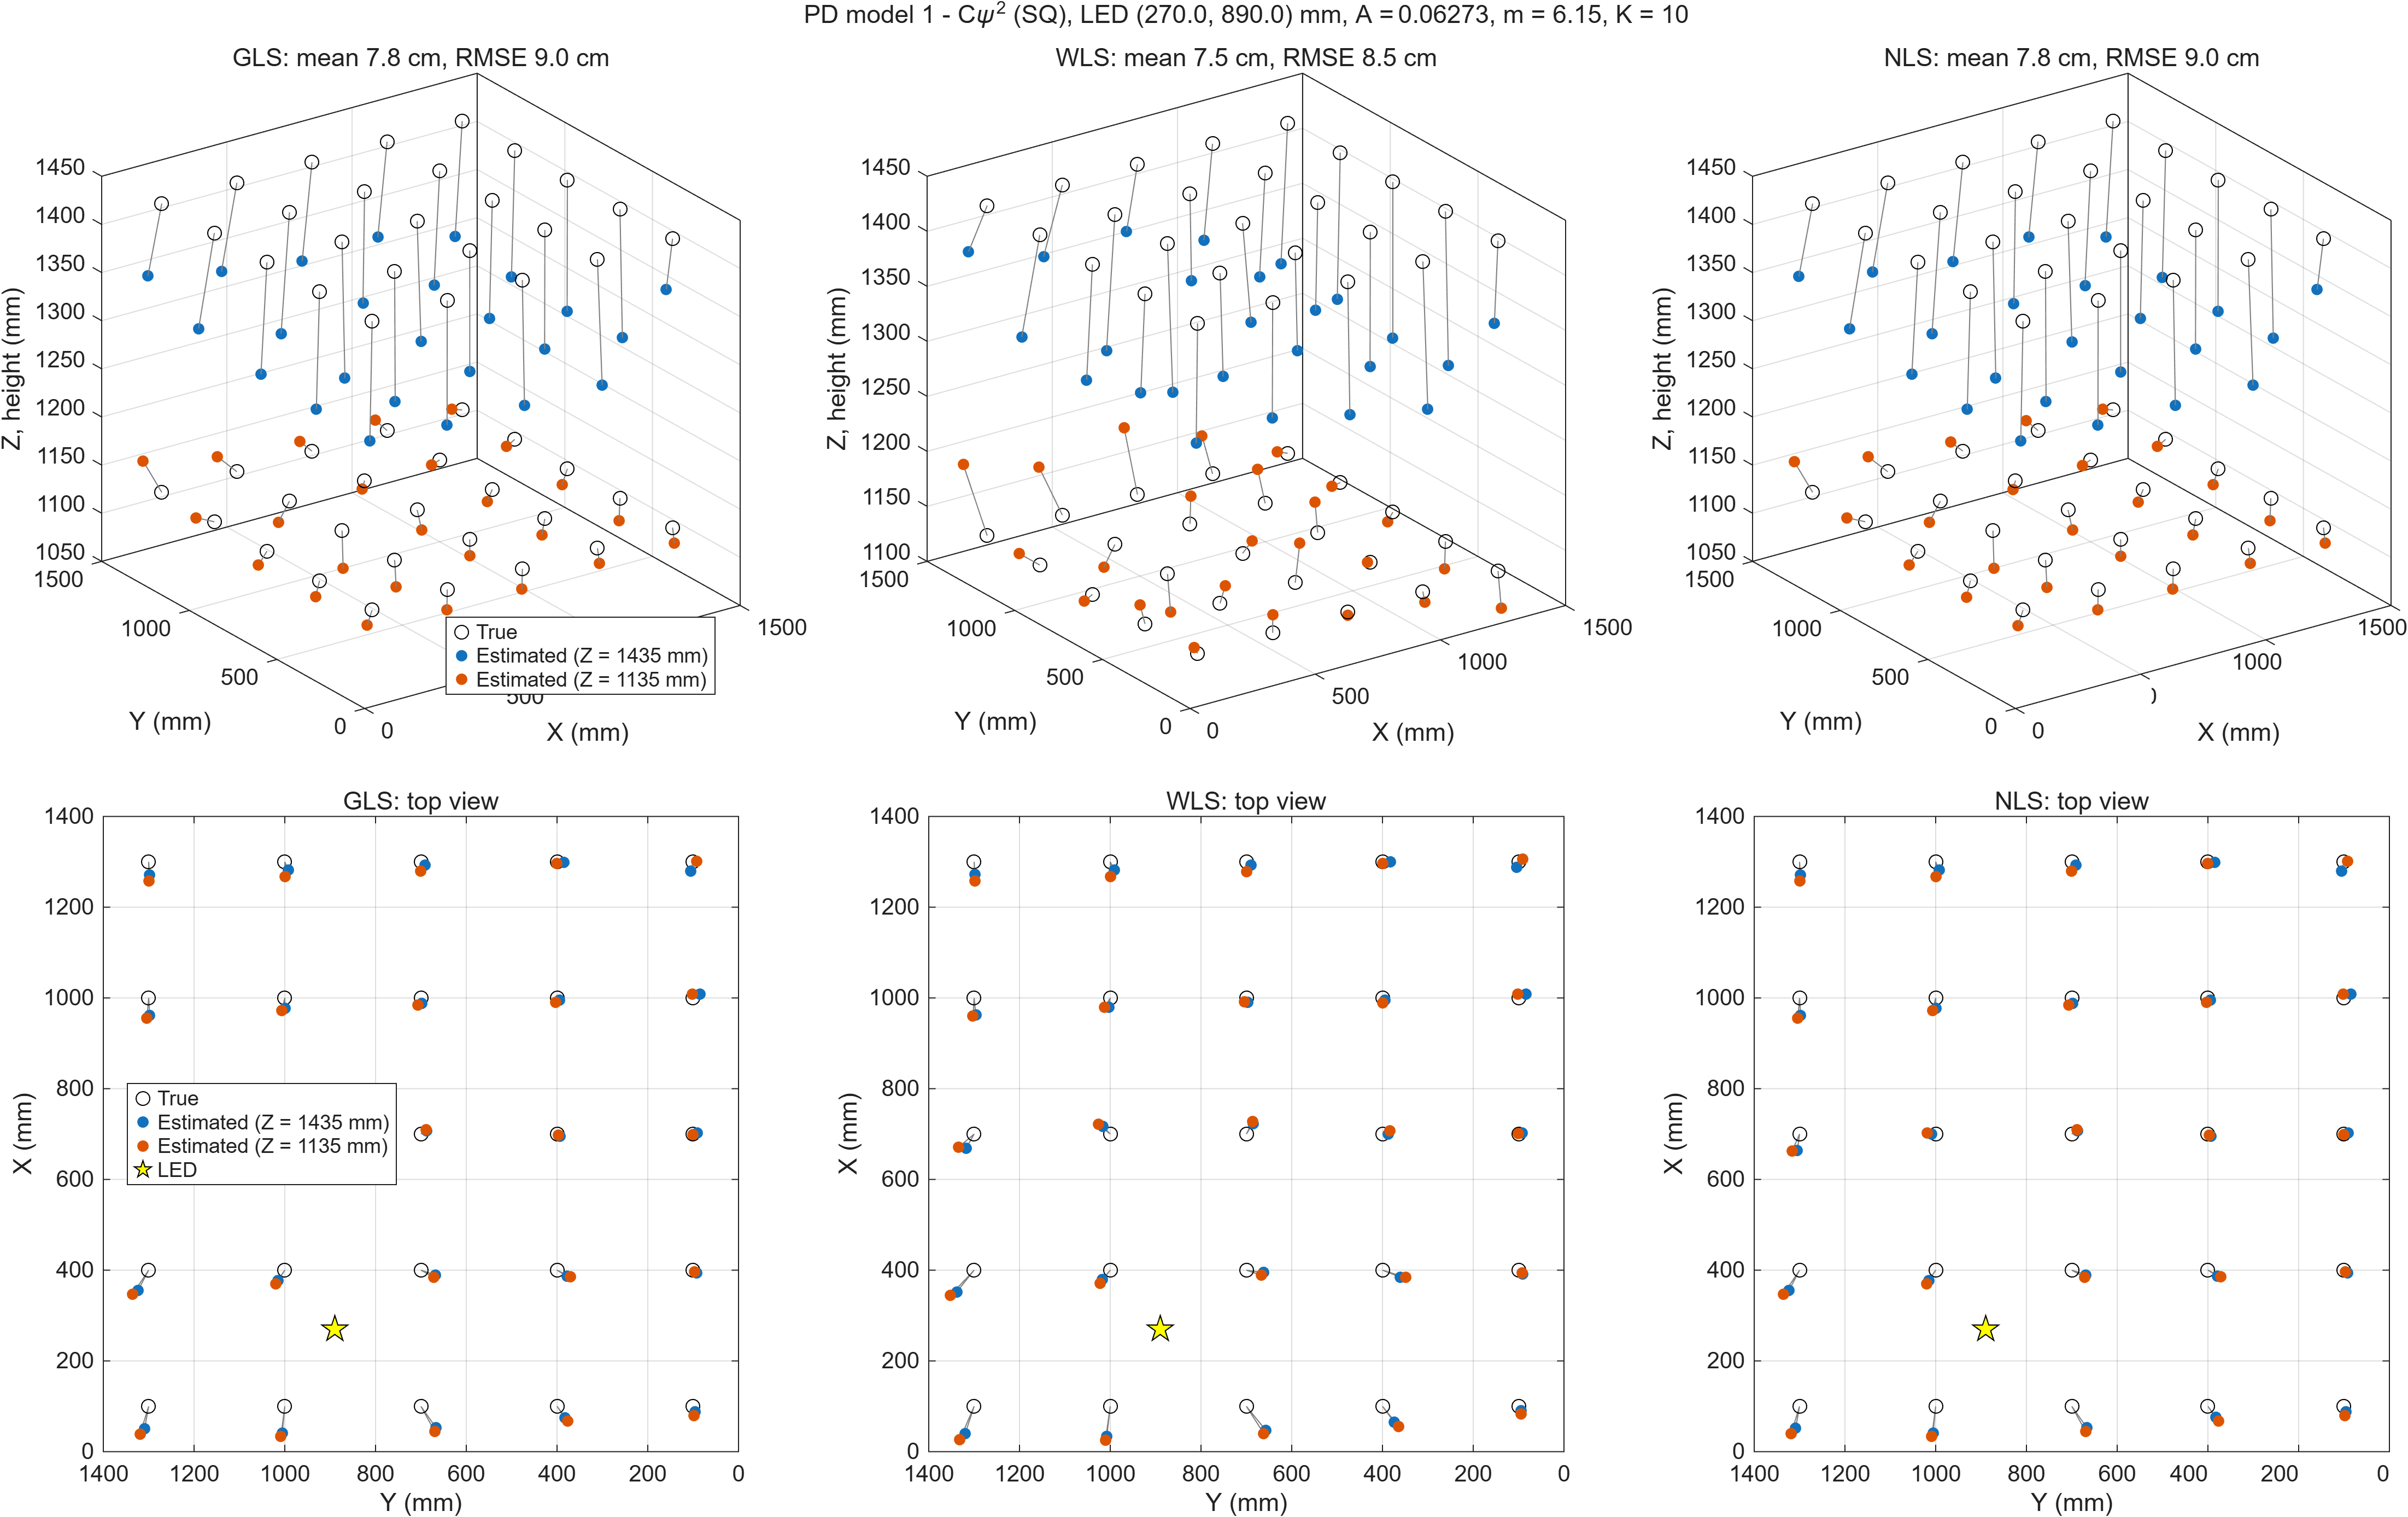
\includegraphics[width=\linewidth]{offset/positions_SQ.png}
\caption{Posiciones verdaderas frente a estimadas (SQ, offset ajustado, geometría nominal). Fila superior: 3D; fila inferior: vista superior con la orientación de la herramienta de adquisición.}
\end{figure}

\section{Diagnóstico del nivel $z=-600$}
\textbf{1. Calibración in situ.} Con las posiciones verdaderas se reajustan $A$ y $m$ en cada nivel: $\ln(y\,d^2/R)=\ln A+m\ln\cos\phi$.
\begin{center}\small
\begin{tabular}{lccc}\toprule
Nivel (SQ) & medida/modelo & $A$ (V\,m$^2$) & $m$\\\midrule
barrido de calibración & -- & 0.0627 & 6.15\\
$z=-300$, $Z=1.135$~m & $1.002\pm0.043$ & 0.0606 & 5.68\\
$z=-600$, $Z=1.435$~m (nominal) & $0.986\pm0.106$ & 0.0536 & 4.80\\
$z=-600$, $Z=1.335$~m ($s_z=0.667$) & $0.998\pm0.044$ & 0.0605 & 5.78\\\bottomrule
\end{tabular}\end{center}
Con la altura nominal, el nivel superior es incompatible con la calibración: $A$ baja un 12~\%, el patrón aparente es más plano y la dispersión se duplica. Con el PD 10~cm más bajo, los dos niveles coinciden.

\textbf{2. Triangulación con sólo las direcciones.} Se buscan por mínimos cuadrados el punto de corte de los rayos $\mathbf r_i+\delta_z\mathbf e_z+t\hat{\mathbf u}_i$ y un desplazamiento vertical $\delta_z$ del nivel $z=-600$. Este resultado no depende de $A$, de $m$ ni de la distancia.
\begin{center}\small
\begin{tabular}{lccc}\toprule
Modelo / est. & LED triangulado (mm, mm, m) & $\delta_z$ del nivel $-600$ & RMS de rayos\\\midrule
SQ, GLS/NLS & (299.3, 886.3, \textbf{2.972}) & $\mathbf{-105}$~mm & 21.2~mm\\
SQ, WLS & (301.6, 885.2, 2.937) & $-118$~mm & 29.9~mm\\
$\cos^{1.9}$, NLS & (298.5, 887.2, 3.030) & $-45$~mm & 43.9~mm\\
SQ, NLS con $s_z=0.667$ & (299.3, 886.3, 2.972) & $-5$~mm & 21.1~mm\\\bottomrule
\end{tabular}\end{center}
Las direcciones sitúan el LED a 2.97~m, casi la altura nominal, y piden bajar el nivel superior unos 10.5~cm. La amplitud da $-11.5$~cm. Ambos principios coinciden: unos 190--200~mm de recorrido real por 300~mm comandados, un factor cercano a 2/3.

\textbf{3. Barrido del recorrido supuesto.} Las estimaciones no dependen de $s_z$, salvo por el ajuste cruzado del offset; lo que cambia es la referencia. El mínimo error medio, 3.3~cm, está en unos 180--185~mm (Fig.~\ref{fig:sweep}).

\begin{figure}[H]\centering
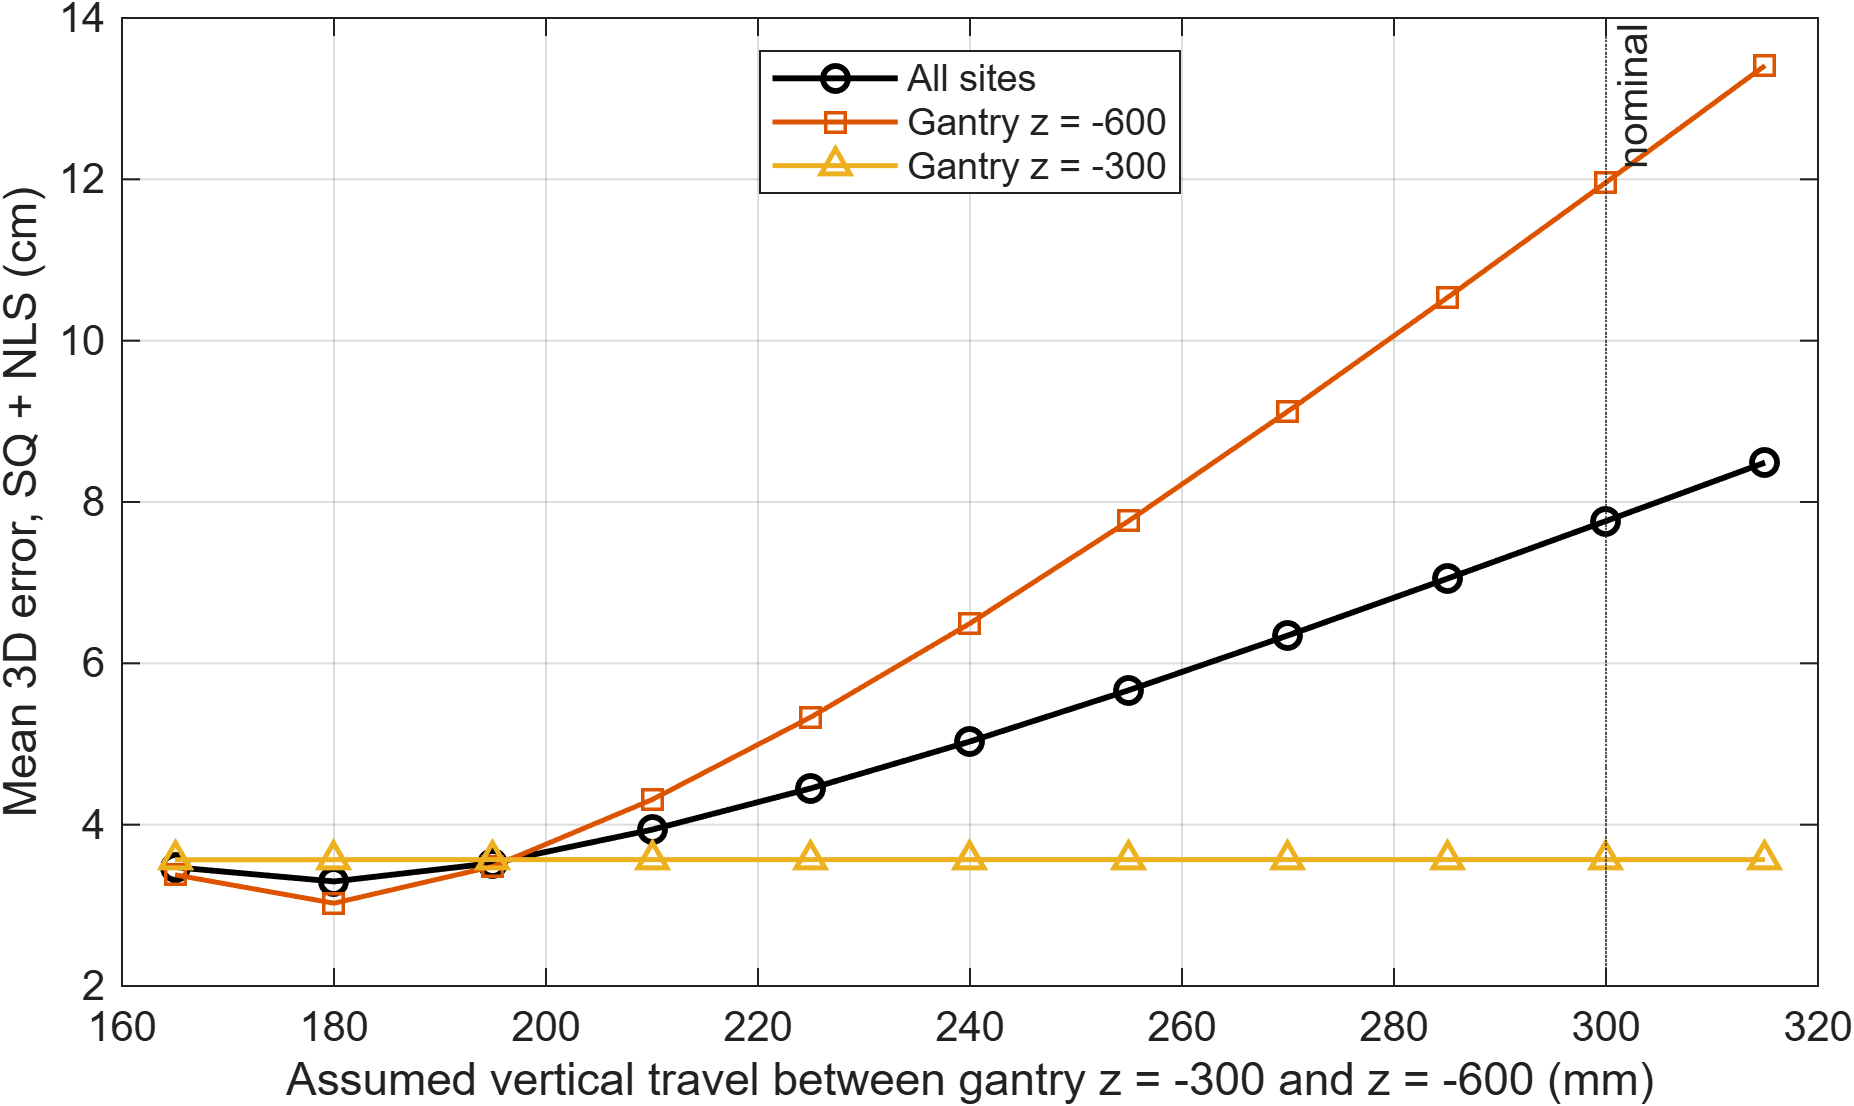
\includegraphics[width=0.72\linewidth]{zscale_sweep.png}
\caption{Error medio (SQ + NLS, offset ajustado) frente al recorrido vertical supuesto entre los dos niveles.}\label{fig:sweep}
\end{figure}

\begin{table}[H]\centering\small
\begin{tabular}{lrrrrrrr}\toprule
Variante (SQ, NLS) & media & RMSE & P90 & $z=-600$ & sesgo & $z=-300$ & sesgo\\\midrule
Nominal ($65^\circ$, $15^\circ$) & 8.58 & 9.52 & 13.94 & 12.39 & $-11.55$ & 4.77 & $-0.92$\\
Offset ajustado (cruzado) & 7.76 & 8.99 & 13.10 & 11.96 & $-11.55$ & 3.57 & $-0.92$\\
Offset + tilt (cruzado) & 10.45 & 10.88 & 14.70 & 10.42 & $-9.86$ & 10.47 & $+8.19$\\
Offset, LED (281.1, 904.8) & 7.79 & 9.10 & 13.64 & 12.23 & $-11.97$ & 3.34 & $-1.30$\\
Offset, elevación campaña 0 & 6.63 & 7.34 & 11.21 & 3.90 & $-1.85$ & 9.37 & $+8.78$\\
Nominal ($65^\circ$), $s_z=0.667$ & 4.83 & 5.01 & 6.44 & 4.88 & $-1.56$ & 4.77 & $-0.92$\\
\textbf{Offset, $s_z=0.667$} & \textbf{3.65} & \textbf{3.92} & \textbf{5.89} & 3.74 & $-1.56$ & 3.57 & $-0.92$\\\bottomrule
\end{tabular}
\caption{Variantes de los hiperparámetros (cm, 50 posiciones). Si la elevación del adaptador de $15^\circ$ fuese 0, se arreglaría el nivel superior a costa del inferior: una elevación común no explica los dos niveles; sólo un recorrido vertical menor lo hace.}\label{tab:variants}
\end{table}

\begin{figure}[H]\centering
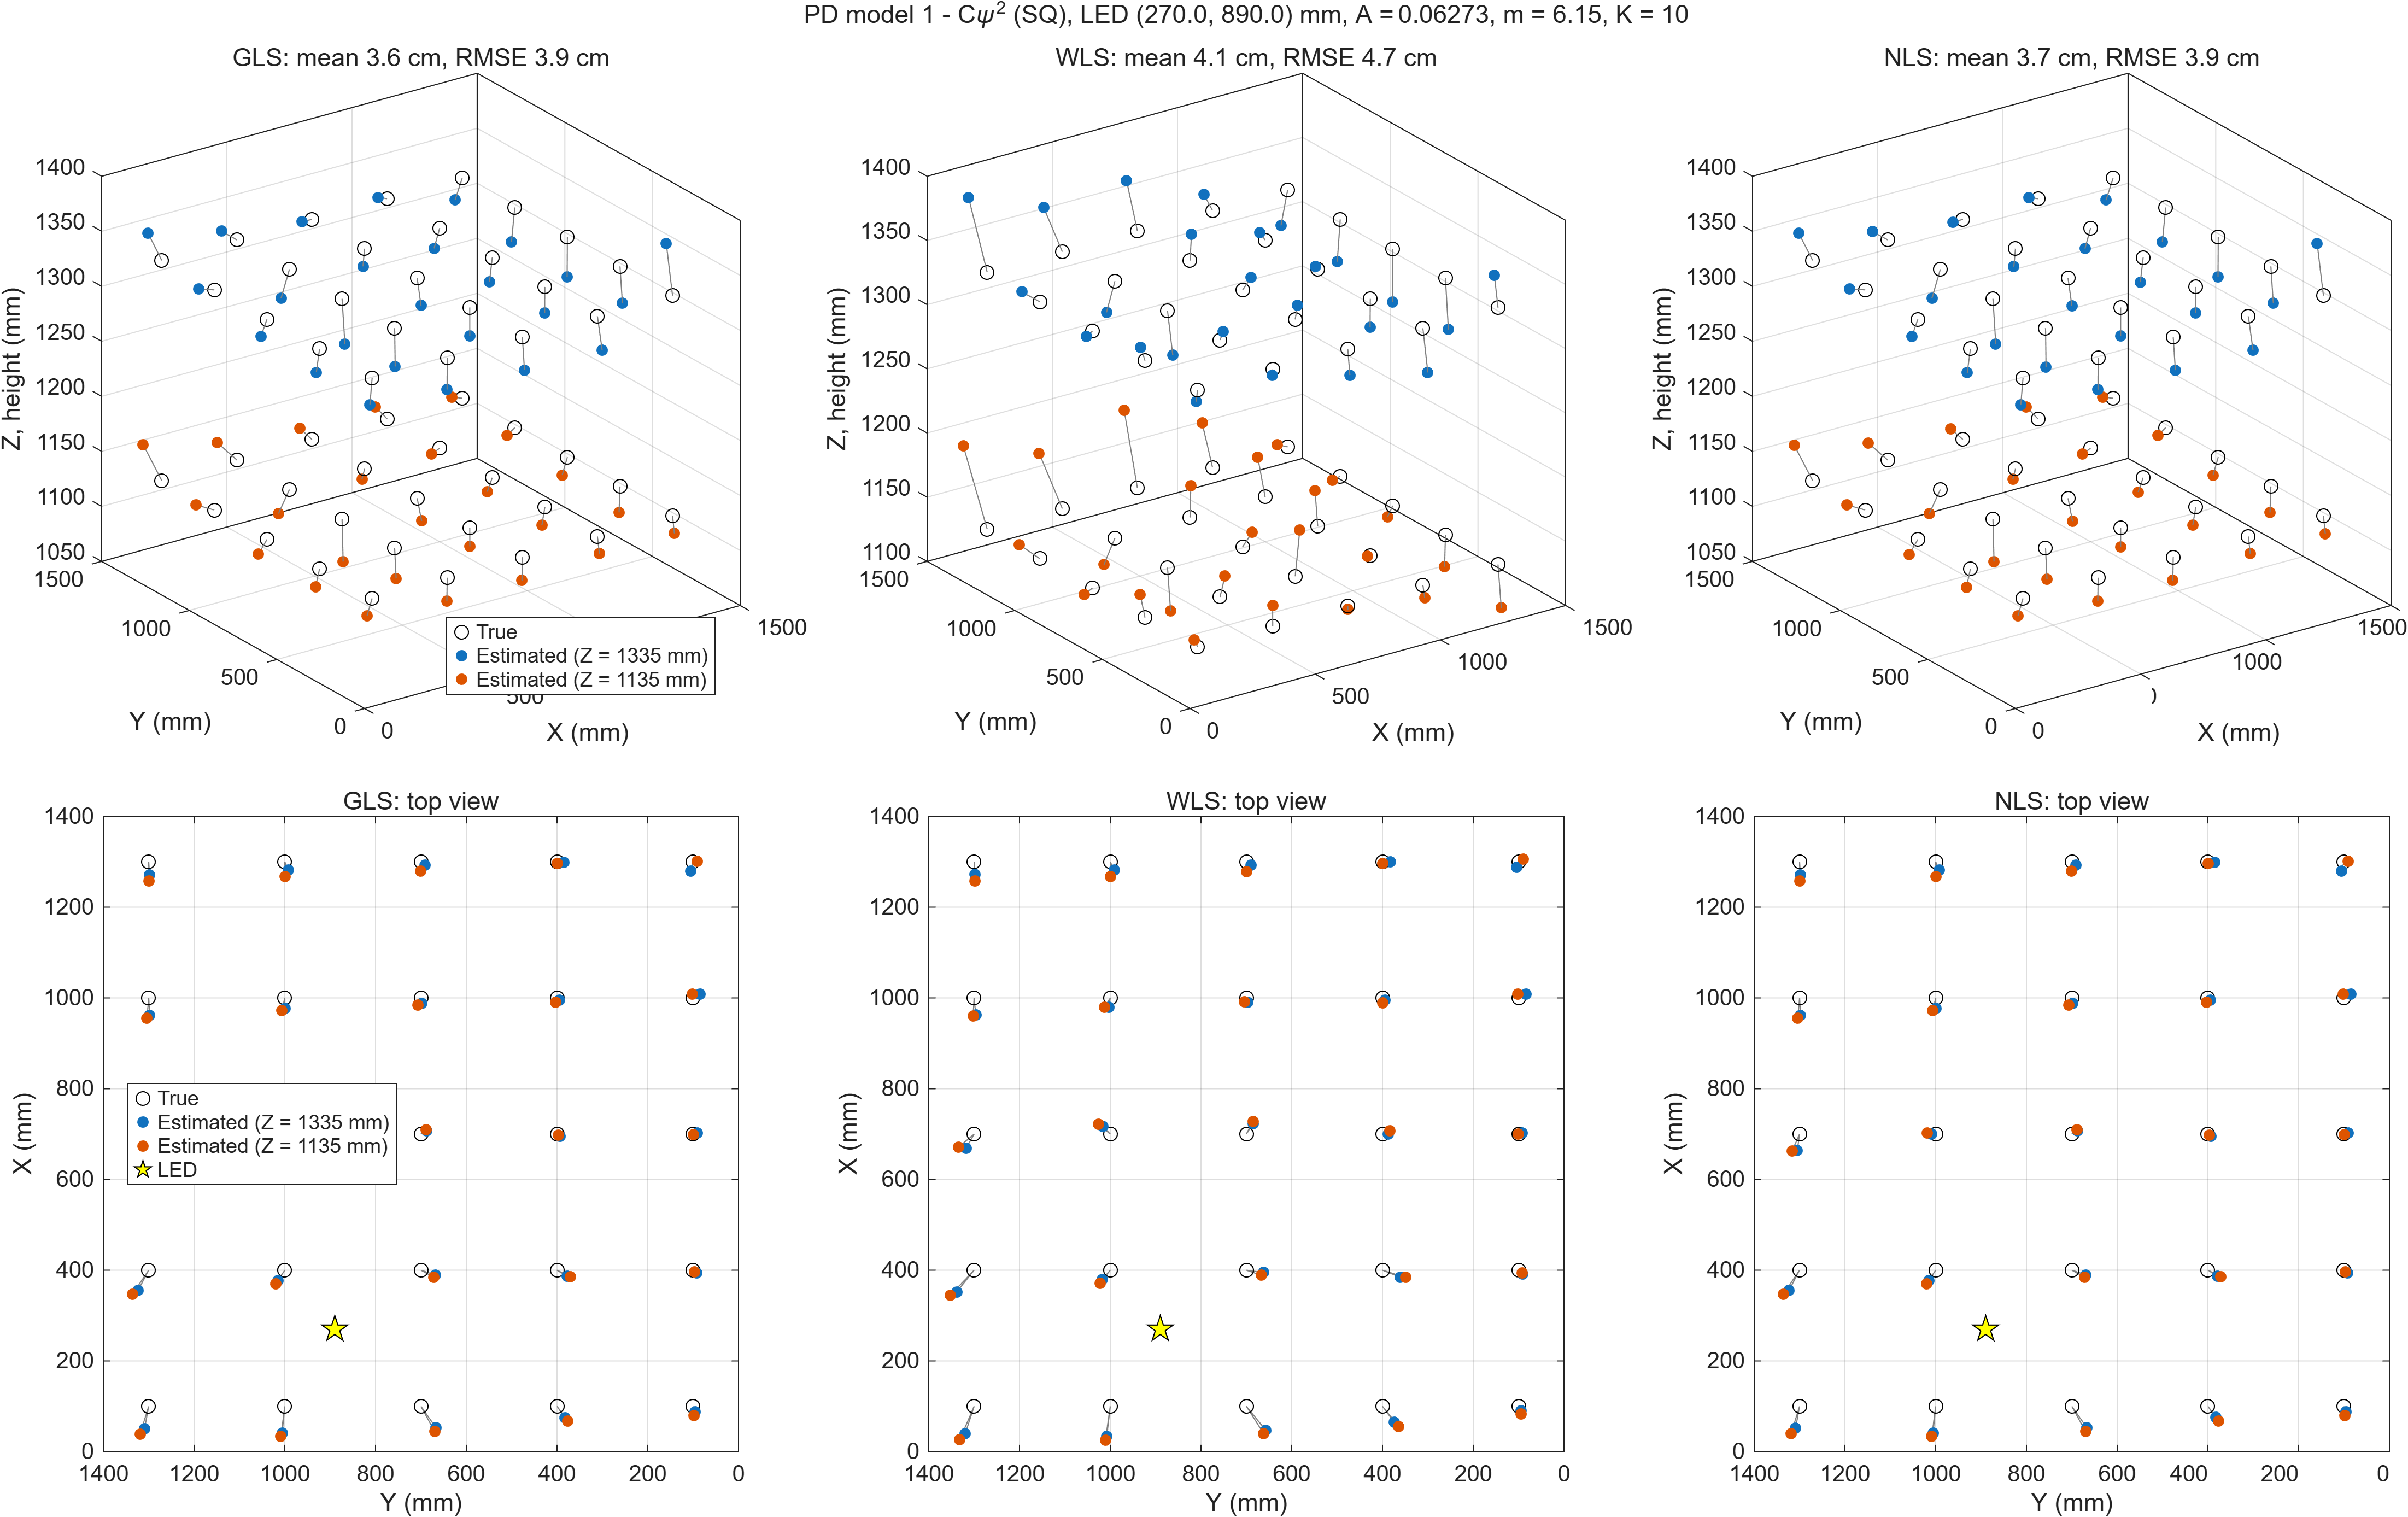
\includegraphics[width=\linewidth]{zscale/positions_SQ.png}
\caption{SQ con offset ajustado y $s_z=0.667$, la hipótesis geométrica: media 3.65~cm, RMSE 3.9~cm.}
\end{figure}

\section{Campaña del 15/10: validación con otras tres alturas}\label{sec:c2}
\textbf{Datos.} \path{campaign_20261015-000723_grid5x5x3-xy100to1300-s300-z-200to0_K10-off65_pd15_tilt0_100ms}: misma rejilla XY, $K=10$ con los mismos ángulos, adaptador de $15^\circ$, gantry $z=-200$, $-100$ y $0$ (00:07--05:23, 750 medidas en 5.27~h, sin recortes). El programa analiza las dos campañas juntas (\path{campaign_dirs}): 125 posiciones en 5 alturas. Los datos están ordenados en el tiempo de $z=-600$ a $z=0$.

\textbf{Geometría nominal: el sesgo es lineal en $z$.}
\begin{center}\small
\begin{tabular}{lrrrrr}\toprule
Gantry $z$ (mm) & $-600$ & $-300$ & $-200$ & $-100$ & $0$\\\midrule
$Z_{\rm PD}$ nominal (m) & 1.435 & 1.135 & 1.035 & 0.935 & 0.835\\
Error medio SQ+NLS (cm) & 11.96 & 3.57 & 4.21 & 7.00 & 10.40\\
Sesgo vertical (cm) & $-11.55$ & $-0.92$ & $+2.64$ & $+6.01$ & $+9.69$\\
Triangulación sólo direcciones, $\delta_z$ (mm) & $-105.6$ & 0 (ref.) & $+39.9$ & $+75.1$ & $+112.9$\\
$A$ in situ (V\,m$^2$) & 0.0536 & 0.0606 & 0.0626 & 0.0644 & 0.0664\\
$m$ in situ & 4.80 & 5.68 & 5.94 & 6.15 & 6.38\\
Tilt ajustado ($^\circ$) & 13.76 & 14.77 & 15.09 & 15.33 & 15.57\\\bottomrule
\end{tabular}\end{center}
Dos principios independientes miden directamente la separación vertical entre niveles:
\begin{itemize}
\item la regresión de las alturas estimadas da \textbf{0.647~mm reales por mm comandado};
\item la triangulación con sólo las direcciones da \textbf{0.632}.
\end{itemize}
Además, con la geometría nominal tanto $A$ y $m$ del LED como el tilt del adaptador \emph{dependerían de la altura del PD}, lo que físicamente no tiene sentido.

\textbf{Con $s_z=0.667$, fijado con la campaña del 14/10.}
\begin{center}\small
\begin{tabular}{lrrrrr}\toprule
Gantry $z$ (mm) & $-600$ & $-300$ & $-200$ & $-100$ & $0$\\\midrule
$Z_{\rm PD}$ (m) & 1.335 & 1.135 & 1.068 & 1.002 & 0.935\\
Error medio SQ+NLS (cm) & 3.75 & 3.57 & 3.72 & 3.70 & 3.71\\
P90 (cm) & 5.55 & 6.40 & 6.62 & 6.99 & 7.15\\
Sesgo vertical (cm) & $-1.56$ & $-0.92$ & $-0.69$ & $-0.65$ & $-0.30$\\
Triangulación, $\delta_z$ (mm) & $-5.7$ & 0 & $+6.6$ & $+8.5$ & $+13.0$\\
$A$ in situ (V\,m$^2$) & 0.0605 & 0.0606 & 0.0606 & 0.0604 & 0.0605\\
$m$ in situ & 5.78 & 5.68 & 5.65 & 5.58 & 5.55\\
Tilt ajustado ($^\circ$) & 14.82 & 14.77 & 14.81 & 14.79 & 14.81\\\bottomrule
\end{tabular}\end{center}
Sin reajustar nada:
\begin{itemize}
\item las cinco alturas tienen el mismo error;
\item $A$ queda constante a $\pm0.2$~\% y coincide con la calibración ($A_{\rm cal}=0.0627$; medida/modelo $=1.000\pm0.042$);
\item el tilt es $14.80\pm0.02^\circ$;
\item la triangulación cierra a $\pm13$~mm.
\end{itemize}
En la campaña nueva, el error es de 3.71~cm de media (RMSE 4.23, P90 6.94). En las 125 posiciones, SQ+NLS da 3.69~cm (RMSE 4.11, P90 6.62) y SQ+GLS 3.68~cm. Con $s_z=1$ el error medio sería de 7.43~cm.

\textbf{Otras observaciones.}
\begin{itemize}
\item \textbf{$\cos^{1.9}$ no es coherente con ninguna geometría}: con $s_z=0.667$ su tilt varía de 15.2 a $14.3^\circ$ y la triangulación deja desplazamientos de $+54$ a $-40$~mm (error medio de 8~cm). Es otra indicación de que SQ es la respuesta correcta de este PD.
\item El offset ajustado deriva de forma monótona con el orden de adquisición: $67.55^\circ$ ($z=-600$, 14/10 a las 19~h) $\to 67.06^\circ$ ($z=0$, 15/10 a las 5~h). Son $0.5^\circ$ en 10~h, quizá del MTRS o del montaje; su efecto es pequeño.
\item El error horizontal (2.6--3.3~cm) es sistemático por posición XY y se repite en todas las alturas, sobre todo en las filas $X\le400$. Con el LED en $(300,885)$, el valor triangulado, baja a 2.4~cm, pero aparece un sesgo vertical de $+1.9$~cm por el cambio de $A$ y $m$; el total no mejora (3.76~cm).
\end{itemize}

\begin{figure}[H]\centering
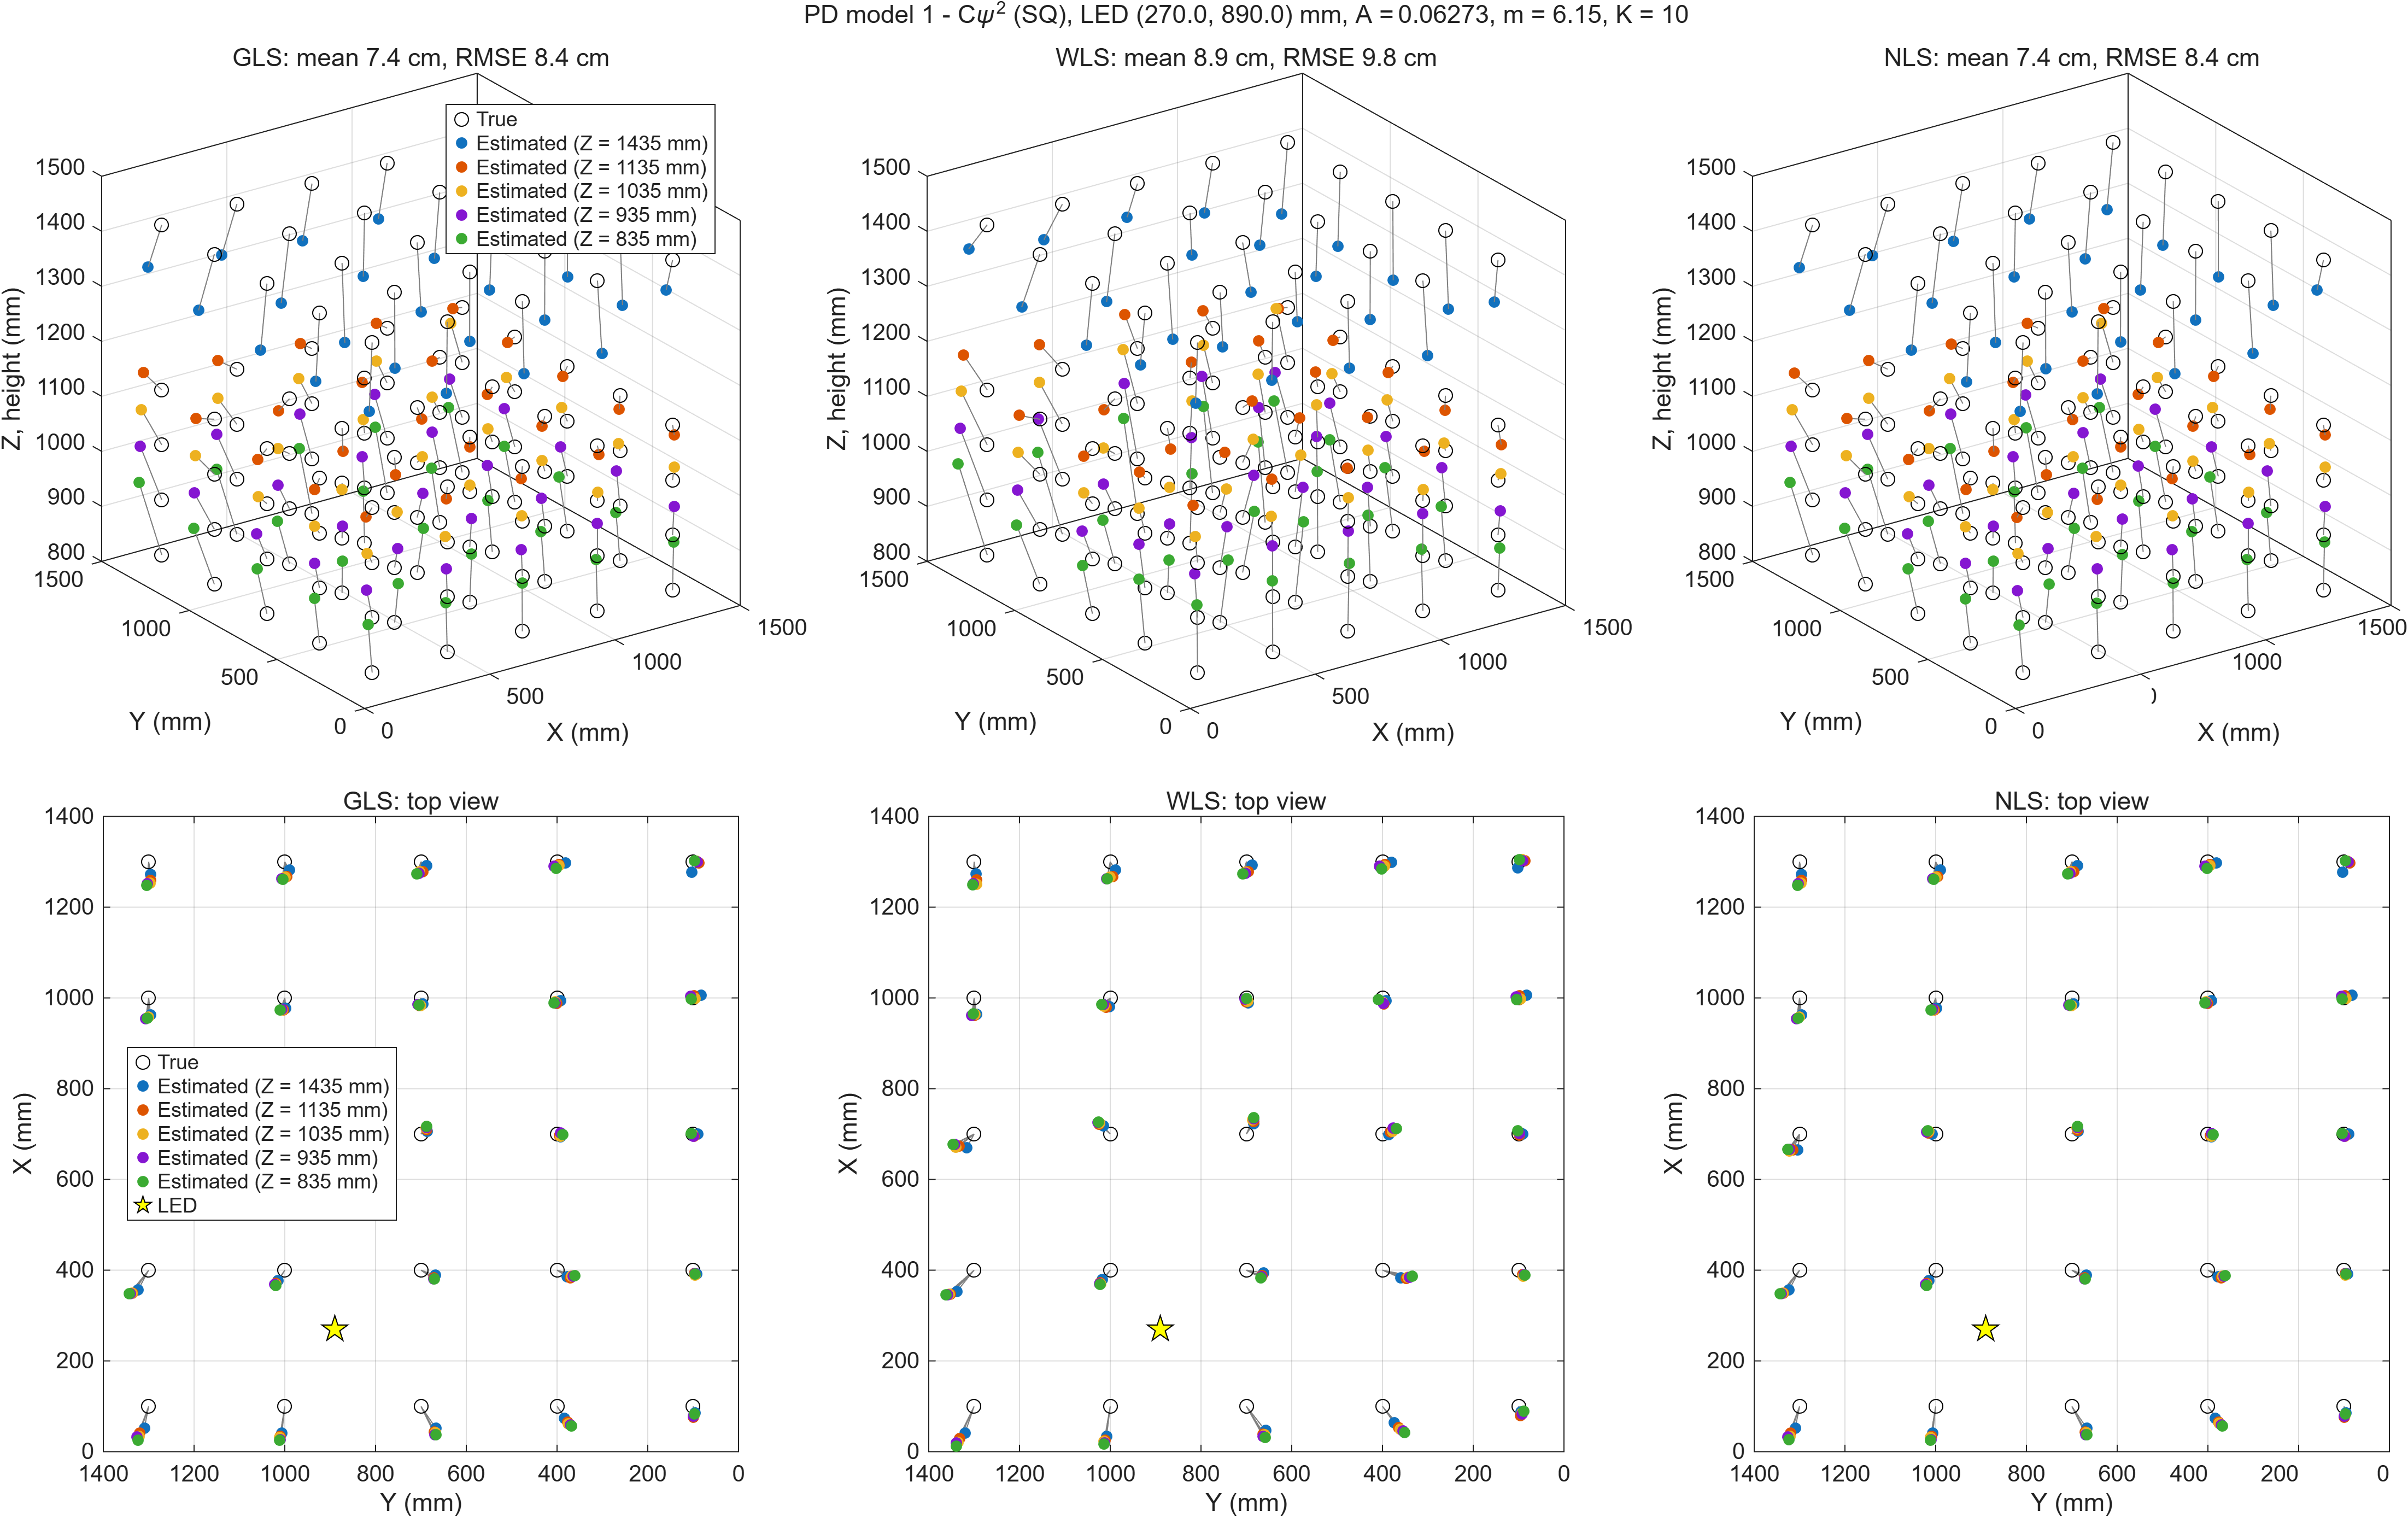
\includegraphics[width=\linewidth]{combined_nominal/positions_SQ.png}
\caption{125 posiciones, SQ, offset ajustado, geometría nominal: el sesgo vertical cambia de signo entre las alturas extremas.}
\end{figure}
\begin{figure}[H]\centering
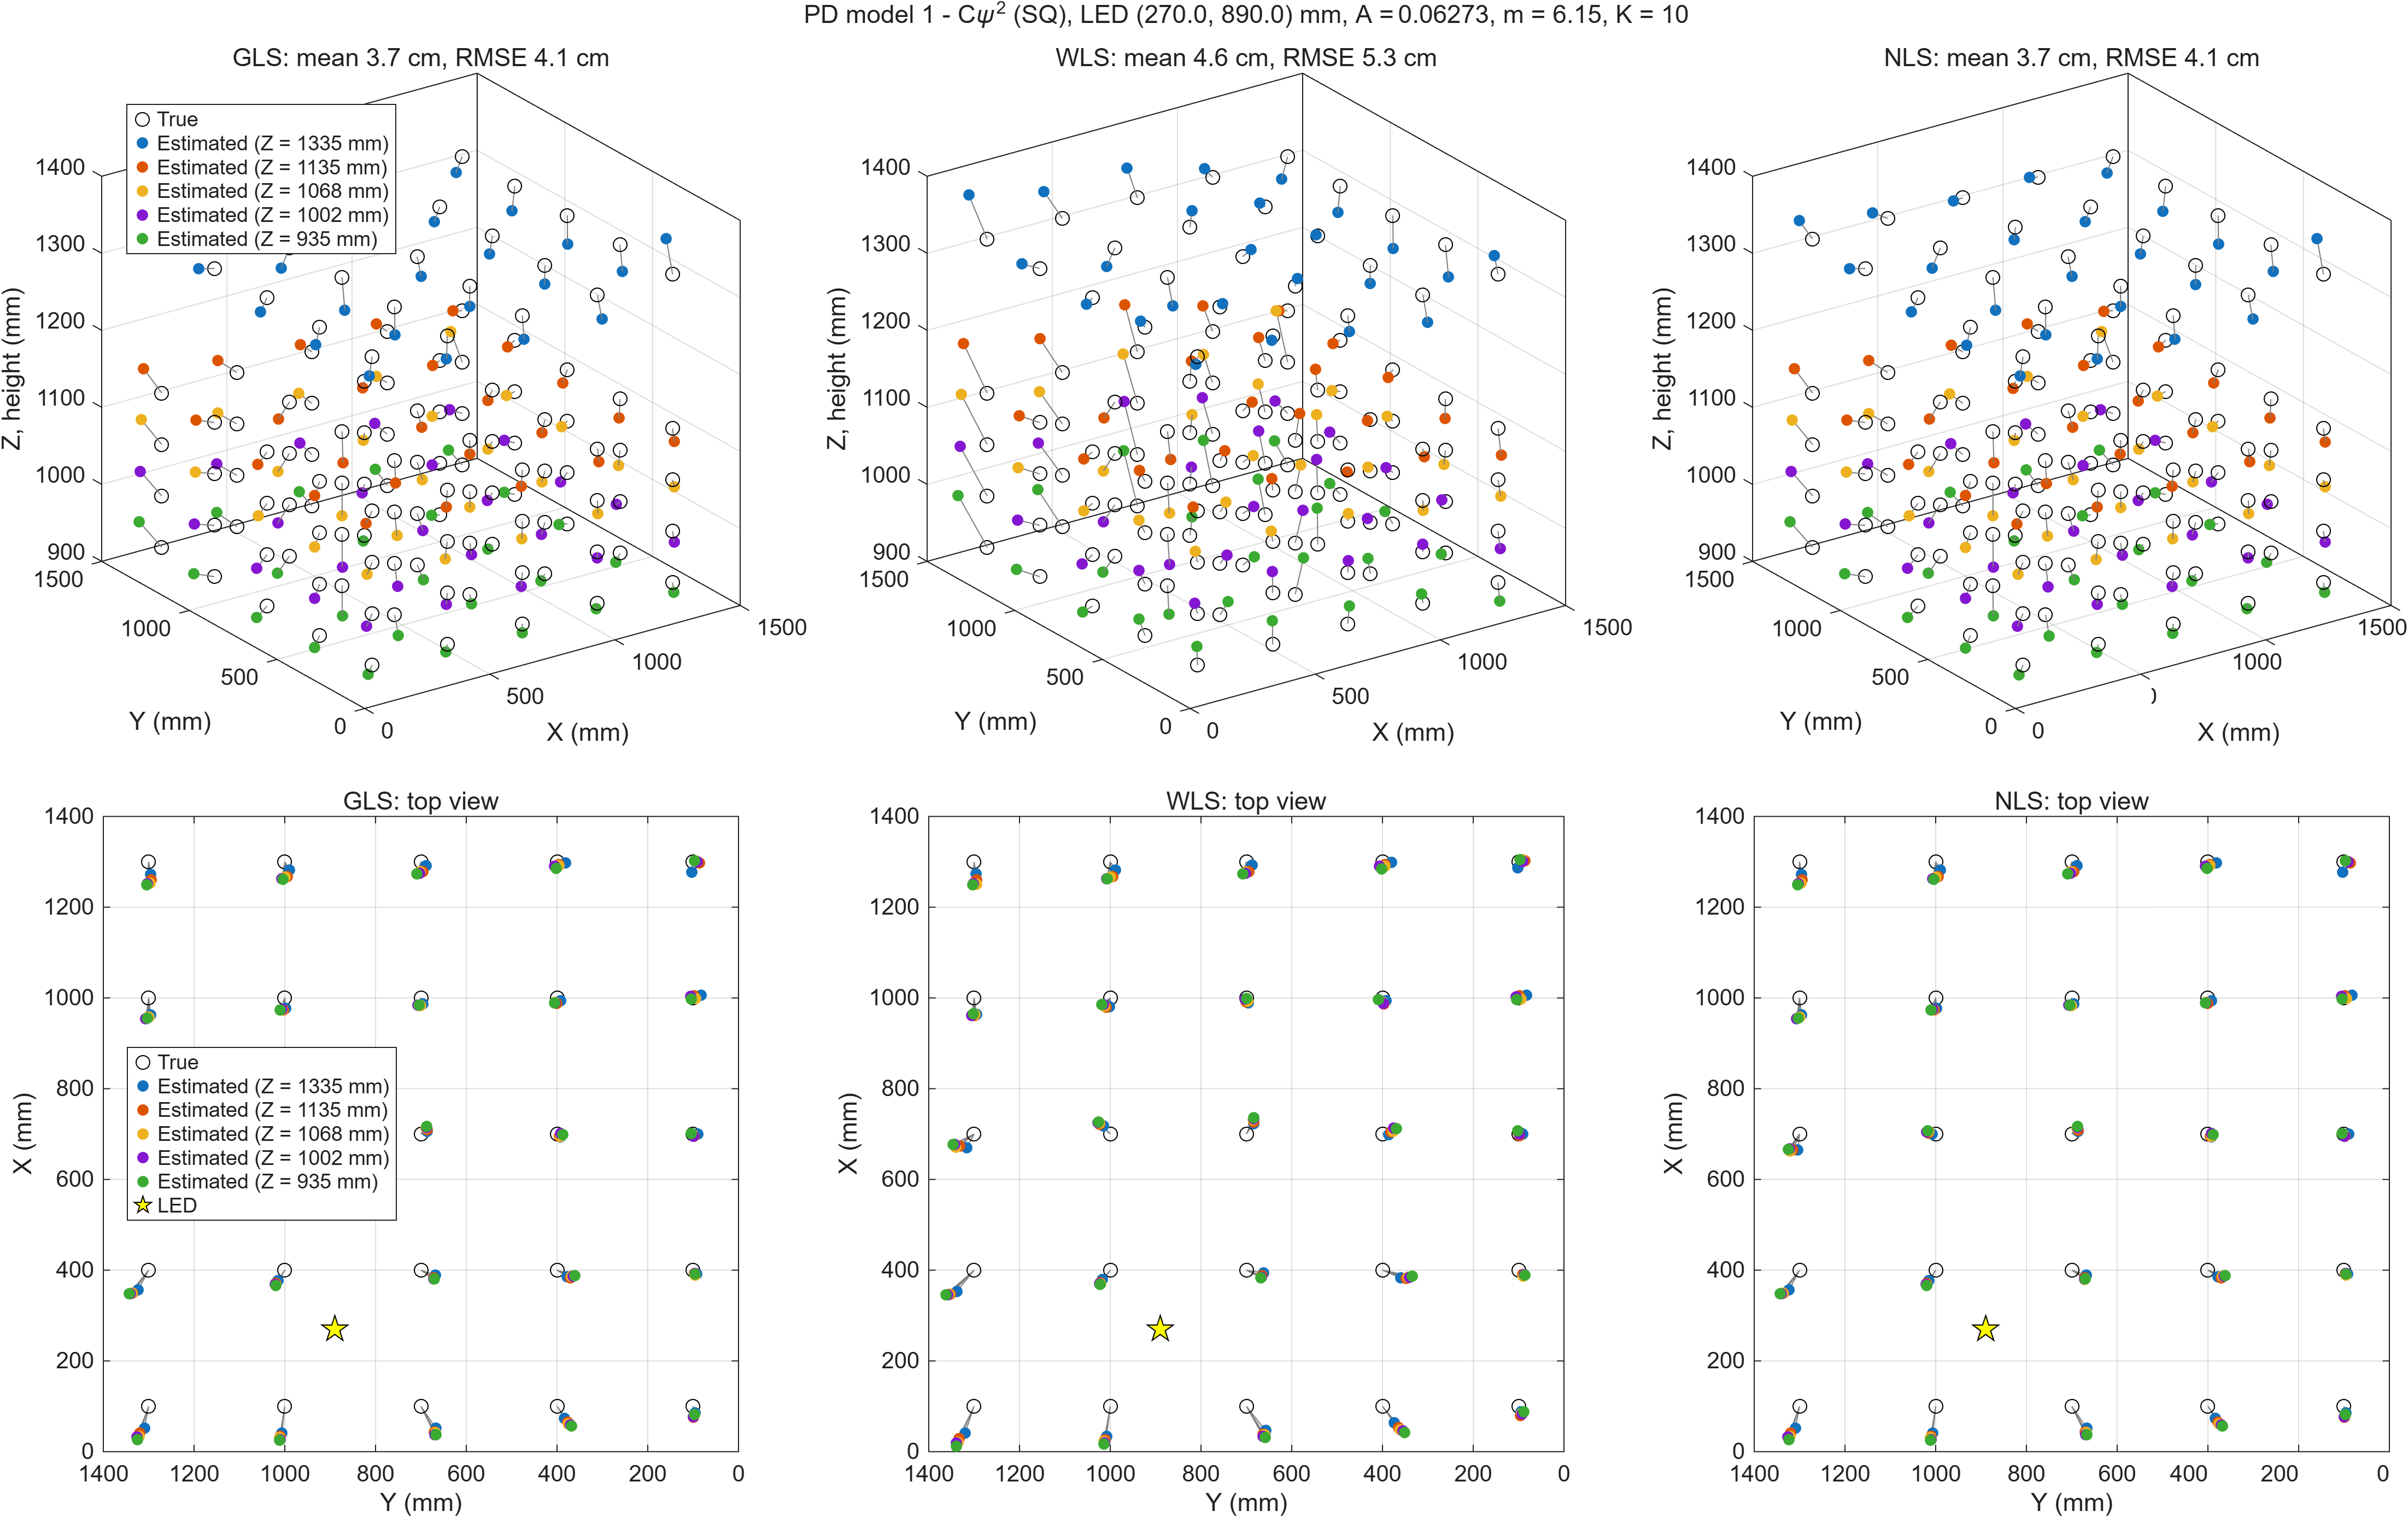
\includegraphics[width=\linewidth]{combined/positions_SQ.png}
\caption{125 posiciones con $s_z=0.667$ (fijado con la primera campaña): media 3.69~cm, RMSE 4.11~cm.}
\end{figure}

\section{Resultados con la geometría medida ($s_z=0.6$)}\label{sec:measured}
\textbf{Medición.} El investigador comprobó con cinta que el recorrido vertical real es 0.6 veces el comandado. Las alturas del PD quedan en $Z=1.315$, 1.135, 1.075, 1.015 y 0.955~m para gantry $z=-600$, $-300$, $-200$, $-100$ y $0$. Éste es ahora el valor por defecto de \path{gantry_z_scale}. Sólo cambia la referencia: las estimaciones no dependen de $s_z$, salvo por el ajuste cruzado del offset.

\begin{table}[H]\centering\small
\begin{tabular}{llrrrrrrrr}\toprule
PD & Est. & ok & media & RMSE & mediana & P90 & horiz. & sesgo vert. & dir. ($^\circ$)\\\midrule
SQ & GLS & 125/125 & 3.91 & 4.30 & 3.42 & 6.73 & 3.02 & $-1.20$ & 0.86\\
SQ & WLS & 125/125 & 4.46 & 5.12 & 3.86 & 8.18 & 3.52 & $+1.03$ & 1.03\\
SQ & NLS & 125/125 & \textbf{3.92} & \textbf{4.30} & 3.44 & 6.73 & 3.01 & $-1.23$ & 0.86\\
$\cos^{1.9}$ & GLS & 125/125 & 8.43 & 9.72 & 8.31 & 12.35 & 3.32 & $-5.20$ & 1.40\\
$\cos^{1.9}$ & WLS & 125/125 & 7.38 & 8.23 & 6.86 & 10.56 & 3.07 & $-5.03$ & 1.27\\
$\cos^{1.9}$ & NLS & 125/125 & 8.42 & 9.68 & 8.31 & 12.37 & 3.31 & $-5.25$ & 1.40\\
$\cos$ & GLS & 115/125 & 72.3 & 82.0 & 66.3 & 131.8 & 18.4 & $+68.1$ & 11.4\\
$\cos$ & WLS & 116/125 & 76.7 & 85.6 & 75.6 & 132.7 & 19.2 & $+72.4$ & 12.1\\
$\cos$ & NLS & 125/125 & 77.4 & 87.6 & 76.9 & 135.6 & 21.3 & $+72.5$ & 11.8\\\bottomrule
\end{tabular}
\caption{Errores en cm, 125 posiciones, $s_z=0.6$, LED $(270,890)$, offset ajustado de forma cruzada entre alturas.}
\end{table}

\begin{table}[H]\centering\small
\begin{tabular}{lrrrrr}\toprule
Gantry $z$ (mm) & $-600$ & $-300$ & $-200$ & $-100$ & $0$\\\midrule
$Z_{\rm PD}$ (m) & 1.315 & 1.135 & 1.075 & 1.015 & 0.955\\
Error medio SQ+NLS (cm) & 3.07 & 3.57 & 4.00 & 4.32 & 4.62\\
P90 (cm) & 6.36 & 6.40 & 6.73 & 7.27 & 7.55\\
Sesgo vertical (cm) & $+0.45$ & $-0.92$ & $-1.36$ & $-1.99$ & $-2.31$\\
Error horizontal (cm) & 2.57 & 2.93 & 3.04 & 3.21 & 3.30\\
Triangulación, $\delta_z$ (mm) & $+14.4$ & 0 & $-0.1$ & $-4.9$ & $-7.1$\\
$A$ in situ (V\,m$^2$) & 0.0619 & 0.0606 & 0.0601 & 0.0596 & 0.0594\\
$m$ in situ & 5.98 & 5.68 & 5.59 & 5.47 & 5.39\\
Tilt ajustado ($^\circ$) & 15.03 & 14.77 & 14.75 & 14.69 & 14.65\\\bottomrule
\end{tabular}
\caption{Por altura, SQ + NLS con $s_z=0.6$. Primera campaña: 3.32~cm (50 posiciones); segunda: 4.31~cm (75 posiciones).}
\end{table}

\textbf{Interpretación.}
\begin{itemize}
\item El valor medido (0.6) está cerca de lo que estimaba el VLP a partir de las RSS: 0.632 por direcciones y 0.647 por alturas estimadas. La diferencia restante es un 3--5~\% del recorrido, equivalente a $\le2.8$~cm en 600~mm. Se ve como un sesgo vertical que pasa de $+0.5$ a $-2.3$~cm al bajar el PD.
\item Este residuo no se corrige con la altura del LED. Variando $H_{\rm LED}$ entre 2.95 y 3.20~m, el mínimo está en 3.00~m (3.92~cm; 4.97~cm con 3.05~m y 5.97~cm con 2.95~m), y la pendiente del sesgo se mantiene en unos 2.8~cm en todos los casos.
\item Lo más probable es el modelo del LED. $m$ in situ cae de 5.98 a 5.39 a medida que el PD se aleja: el patrón aparente es más plano lejos, algo que $\cos^m$ con un solo $m$ no puede reproducir. Ya el barrido lambertiano mostraba que el LED es más puntiagudo cerca del eje que $\cos^m$. $A$ varía sólo un $\pm2$~\% y el tilt $\pm0.2^\circ$.
\item El LED en $(281.1,904.8)$, la posición \path{joint_xy}, mejora el resultado con la geometría medida: 3.66~cm (RMSE 3.96, P90 6.06, horizontal 2.46~cm). La dispersión medida/modelo también baja, de $\pm0.038$ a $\pm0.022$ a $z=-600$. El offset ajustado pasa entonces a $66.5^\circ$, porque el offset y la posición XY del LED están correlacionados.
\item Otras variantes con $s_z=0.6$ (SQ + NLS):
  \begin{itemize}
  \item offset nominal de $65^\circ$: 4.98~cm;
  \item offset y tilt ajustados de forma cruzada: 3.82~cm;
  \item calibración conjunta de $A$ y $m$: 4.24~cm.
  \end{itemize}
\end{itemize}

\begin{figure}[H]\centering
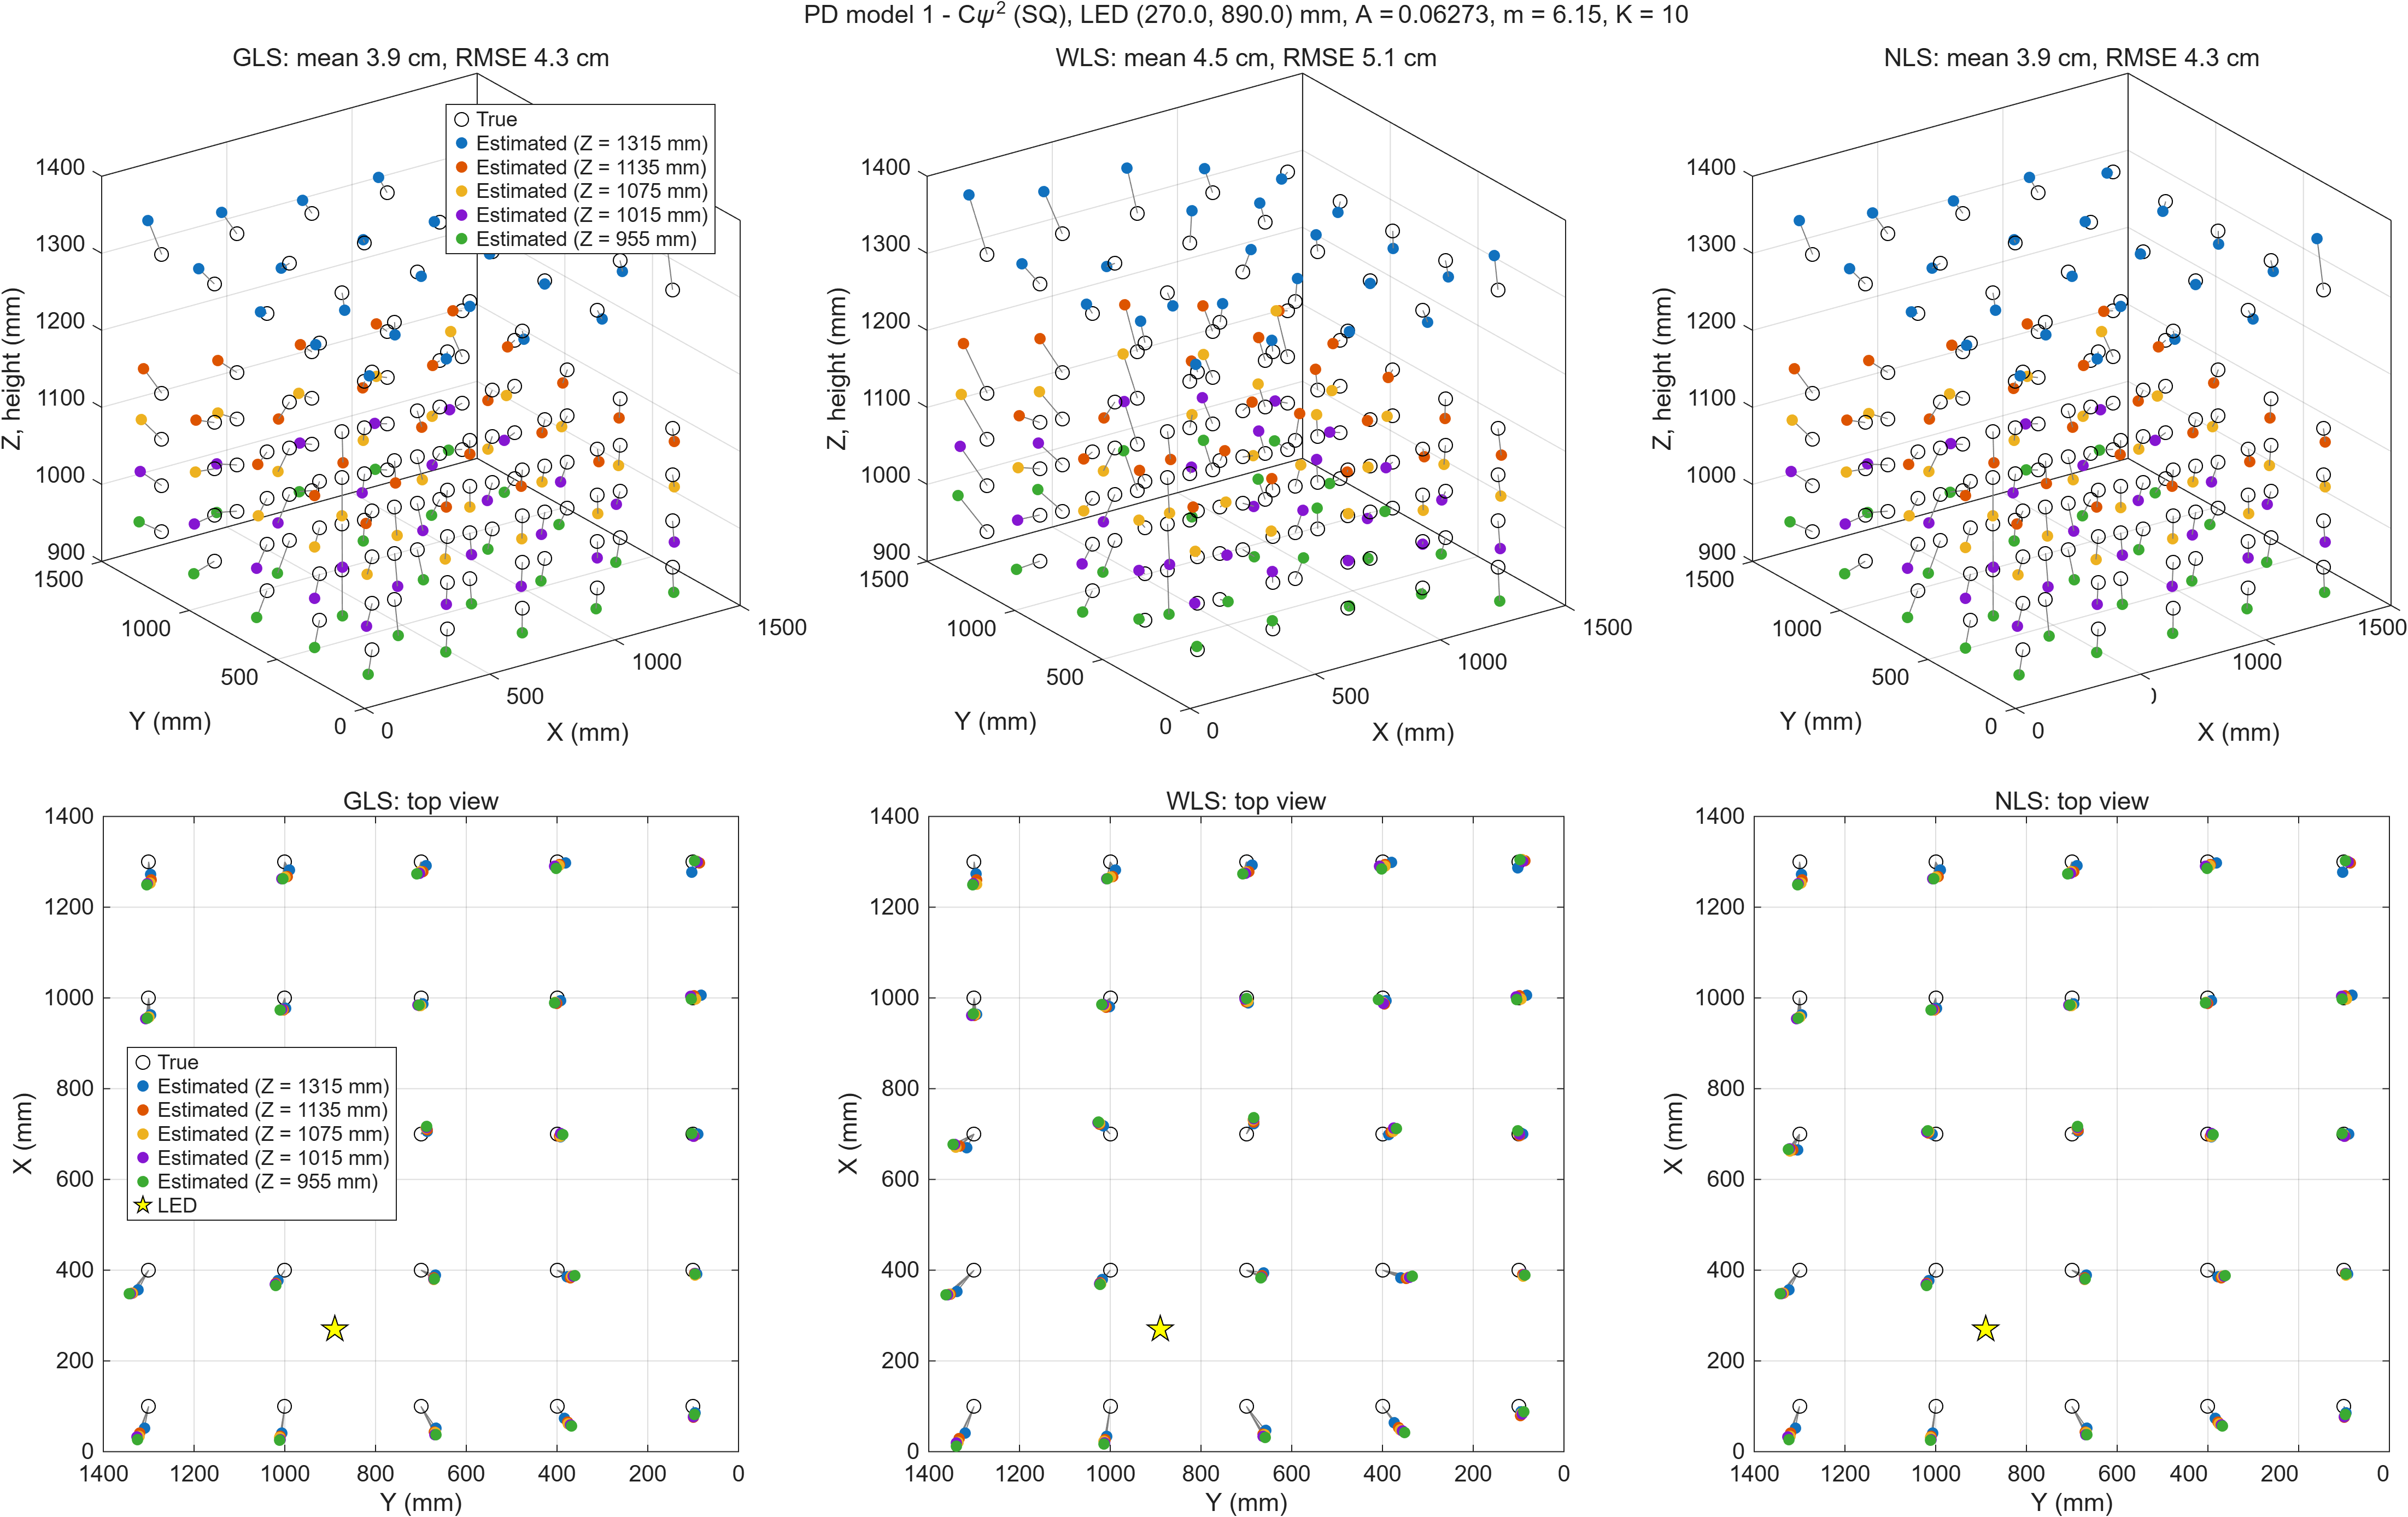
\includegraphics[width=\linewidth]{measured/positions_SQ.png}
\caption{125 posiciones con la geometría medida ($s_z=0.6$), SQ, offset ajustado: media 3.9~cm, RMSE 4.3~cm.}
\end{figure}

\section{Error frente a $K$}
\textbf{Configuración.} SQ + NLS, $s_z=0.6$ (medido), LED $(270,890)$, $A$ y $m$ de la calibración, las 125 posiciones de las dos campañas. Para cada $K$ se usan los subconjuntos casi uniformes de los 10 ángulos medidos, índices $\mathrm{round}(j\cdot10/K)$ para $j=0,\ldots,K-1$, con todas sus rotaciones. Así:
\begin{itemize}
\item $K=3$ son $\{0^\circ,108^\circ,252^\circ\}$, con separaciones de 108, 144 y $108^\circ$, en 10 rotaciones;
\item $K=5$ son dos subconjuntos exactos de $72^\circ$;
\item $K=10$ es el conjunto completo.
\end{itemize}
Se comparan dos casos:
\begin{itemize}
\item \textbf{sin offset:} el valor nominal de $65^\circ$, sin ningún ajuste;
\item \textbf{con offset:} el offset calibrado \emph{una sola vez} con $K=10$ y fijo para todo $K$. Es cruzado entre alturas: cada altura usa el offset ajustado con las otras cuatro.
\end{itemize}

\begin{figure}[H]\centering
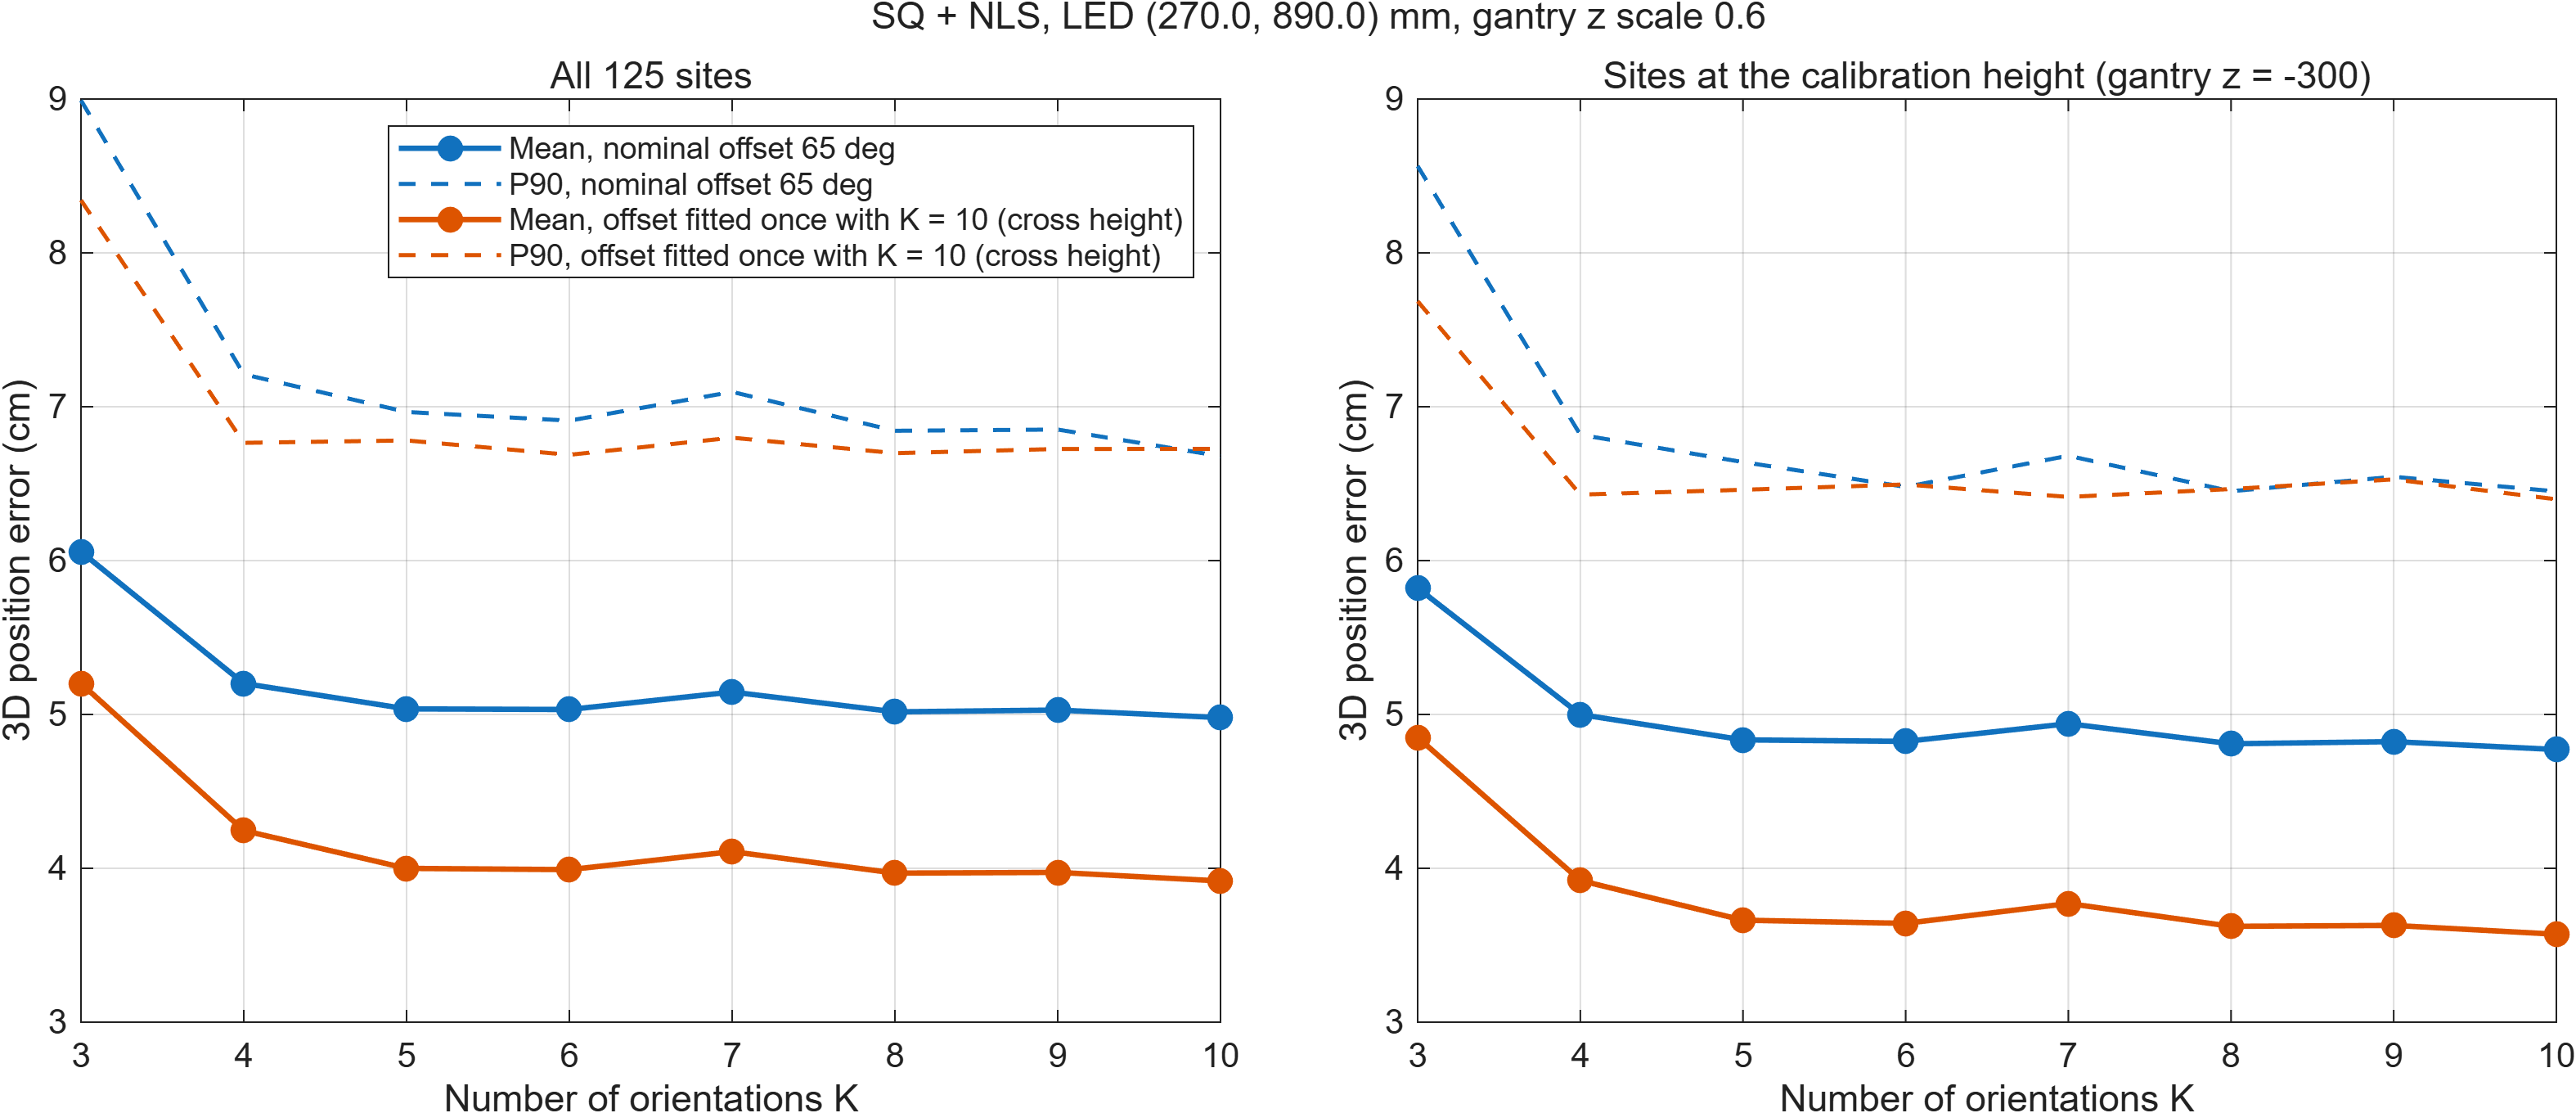
\includegraphics[width=\linewidth]{measured/error_vs_K.png}
\caption{Error 3D medio (continuo) y P90 (discontinuo) frente a $K$, geometría medida. Izquierda: las 125 posiciones. Derecha: sólo el nivel de calibración, que no depende de $s_z$.}\label{fig:K}
\end{figure}

\begin{table}[H]\centering\small
\begin{tabular}{rrrrrrrr}\toprule
 & & \multicolumn{3}{c}{sin offset ($65^\circ$)} & \multicolumn{3}{c}{offset fijo de $K=10$}\\\cmidrule(lr){3-5}\cmidrule(lr){6-8}
$K$ & subconj. & media & P90 & $z=-300$ & media & P90 & $z=-300$\\\midrule
3 & 10 & 6.06 & 8.99 & 5.82 & 5.20 & 8.34 & 4.85\\
4 & 5 & 5.20 & 7.21 & 5.00 & 4.25 & 6.77 & 3.92\\
5 & 2 & 5.04 & 6.97 & 4.83 & 4.00 & 6.78 & 3.66\\
6 & 5 & 5.03 & 6.91 & 4.82 & 3.99 & 6.69 & 3.64\\
7 & 10 & 5.15 & 7.10 & 4.94 & 4.11 & 6.80 & 3.77\\
8 & 5 & 5.02 & 6.84 & 4.81 & 3.97 & 6.70 & 3.62\\
9 & 10 & 5.03 & 6.85 & 4.82 & 3.97 & 6.73 & 3.63\\
10 & 1 & 4.98 & 6.68 & 4.77 & 3.92 & 6.73 & 3.57\\\bottomrule
\end{tabular}
\caption{Error 3D (cm) frente a $K$ con $s_z=0.6$ (subconjuntos $\times$ 125 posiciones). Ningún caso falla, ni siquiera con $K=3$. Con $s_z=0.667$ las curvas eran casi iguales, unos 0.2~cm más bajas.}
\end{table}
\begin{itemize}
\item \textbf{A partir de $K=5$ el error es prácticamente el de $K=10$}: menos de 0.1~cm de diferencia en la media. Las orientaciones adicionales no reducen un error que ya está dominado por los sesgos del modelo y la geometría, no por el ruido.
\item $K=4$ añade 0.2--0.3~cm y $K=3$ cerca de 1~cm. El P90 crece más, porque con $K=3$ el problema está exactamente determinado (3 ecuaciones, 3 incógnitas) y no hay redundancia frente a los sesgos.
\item El offset calibrado una vez reduce el error unos 1.1~cm con cualquier $K$: es un sesgo sistemático, no se compensa con más orientaciones.
\item El panel del nivel $z=-300$ da la misma curva, así que la conclusión sobre $K$ no depende de la hipótesis $s_z$.
\end{itemize}

\section{Conclusiones y próximos pasos}
\begin{enumerate}
\item Los estimadores son los de las simulaciones. La recuperación de distancia es el dual exacto de \path{broadcast_distance}, y con NLS es la MV de la posición.
\item La convención $[\sin t\sin a,\sin t\cos a,\cos t]$ con giro $+Y\to+X$ queda verificada. El offset real es de unos $67.3^\circ$, con una deriva de $0.5^\circ$ en 10~h. Con la geometría corregida, la inclinación es $14.8^\circ$ en las cinco alturas.
\item SQ $>$ $\cos^{1.9}$ $\gg$ $\cos$. GLS $\approx$ NLS; WLS es algo peor. Sólo SQ hace coherentes $A$, el tilt y la triangulación entre alturas.
\item \textbf{El recorrido Z del gantry es 0.6 veces el comandado}, medido con cinta. El VLP lo había detectado sólo con las RSS (0.63--0.65), y la segunda campaña lo confirmó antes de la medición. La configuración del eje Z del gantry afecta a todos los experimentos con Z.
\item \textbf{Resultado final, geometría medida:} SQ + NLS (o GLS), $K=10$, 125 posiciones en 5 alturas, error 3D medio de \textbf{3.9~cm} (RMSE 4.3, P90 6.7~cm), sin fallos. Sin calibrar el offset, 5.0~cm.
\item El error crece suavemente al reducir $K$: con $K=5$ se queda en 4.0~cm y con $K=3$ sube a 5.2~cm (6.1~cm sin offset).
\item \textbf{Siguientes mejoras:}
\begin{itemize}
\item modelar mejor el patrón del LED, cuyo $m$ aparente cambia con la distancia y deja un residuo vertical de unos 2.8~cm en 600~mm (un barrido de calibración a otra altura lo resolvería);
\item medir la posición XY del LED con una plomada: $(281,905)$ da 3.7~cm y la triangulación da $\approx(300,885)$~mm;
\item medir el offset del MTRS en lugar de calibrarlo con los datos.
\end{itemize}
\end{enumerate}

\appendix
\section{Hiperparámetros del programa}
En \path{estimate_3d_positions.m}:
\begin{itemize}\small
\item Datos: \path{campaign_dirs} (carpetas analizadas juntas).
\item LED: \path{led_xy_mm} ([270 890], [281.1 904.8] o 'fit'), \path{H_led_m}.
\item Alturas del PD: \path{H_base_cal_m}, \path{pd_elevation_cal_m}, \path{pd_elevation_m}, \path{gantry_z_scale}.
\item Orientación nominal: \path{mtrs_offset_deg}, \path{pd_tilt_deg}.
\item Calibración de la orientación: \path{orientation_fit} ('none', 'offset', 'offset\_tilt') y \path{orientation_sites} ('all', 'cross\_height').
\item Modelos: \path{calibration_method}, \path{pd_models}, \path{methods}.
\item Estudio frente a $K$: \path{k_study}, \path{k_study_values}, \path{k_study_model}, \path{k_study_method}.
\end{itemize}
\end{document}
